%% cost-of-national-pricing.tex
%% Complete draft formatted for Energy Economics (Elsevier elsarticle).
%% Author-name (Harvard) citations via elsarticle-harv,
%% bound to references.bib.
%%
%% Compile: pdflatex -> bibtex -> pdflatex -> pdflatex
%% Requires: references.bib in the same directory.
%% Empirical figures in Table 1 are produced by run_paper.py.

\documentclass[review,3p,times]{elsarticle}

\usepackage{amsmath,amssymb,amsthm}
\usepackage{booktabs}
\usepackage{graphicx}
\usepackage{url}
\usepackage{xcolor}
\newcommand{\rev}[1]{\textcolor{red}{FM: #1}}
\usepackage{tikz}
\usetikzlibrary{arrows.meta,positioning,shapes.geometric,calc,fit,backgrounds}
\usepackage{pgfplots}
\pgfplotsset{compat=1.18}
\usepgfplotslibrary{groupplots}

\newcommand{\TBD}{\textcolor{red}{[TBD]}}

\theoremstyle{plain}
\newtheorem{proposition}{Proposition}
\theoremstyle{definition}
\newtheorem{definition}{Definition}
\newtheorem{remark}{Remark}
\newtheorem{example}{Example}

\journal{Energy Economics}

\begin{document}

\begin{frontmatter}

\title{The Cost of National Pricing: Side Payments and Efficiency under
Self-Dispatch with Redispatch in the GB Electricity Market}

\author[essex]{Felipe Maldonado\corref{cor}}
\ead{felipe.maldonado@essex.ac.uk}
\cortext[cor]{Corresponding author.}

\address[essex]{School of Mathematics, Statistics and Actuarial Science, University of Essex,
Colchester CO4 3SQ, United Kingdom}

\begin{abstract}
Liberalised electricity markets resolve the nonconvexities created by
generation commitment through out-of-market side payments whose magnitude and
opacity concern regulators. Most analyses adopt the centralised, nodal-dispatch
institution of US independent system operators (ISOs), in which these appear as make-whole
payments on top of locational prices. Great Britain (GB) occupies the opposite
institutional corner: a single national uniform price cleared under
self-dispatch, with network constraints and locked-in commitment resolved
afterwards through redispatch in the Balancing Mechanism, the net cost of which
is \emph{socialised} -- recovered uniformly from demand through balancing charges
rather than charged to the parties that cause it. Following the 2025 Review of Electricity Market
Arrangements (REMA), which retained national pricing and rejected locational
pricing, the policy-relevant question is the cost of that choice. We formalise
GB arrangements as a two-stage market -- a network-blind national clearing
followed by a cost-minimising redispatch -- and prove two central results. First, in a
convex economy national-pricing-with-redispatch is welfare-equivalent to nodal
pricing, so every unit of realised welfare loss is attributable to commitment
nonconvexity. Second, the visible cost of national pricing decomposes into a
congestion-rent component that nodal pricing would internalise as merchandising
surplus (the standard term for the network revenue an ISO collects from pricing
energy differently on the two sides of a binding constraint), plus a strategic
redispatch markup; we show this gap is non-negative
under the empirically supported condition that minimised nodal make-whole
payments are small. We quantify the gap on the Scotland--England (B6) boundary
using public Balancing Mechanism data, exploiting the exact correspondence
between the model's two stages and the settlement objects (final physical
notifications and flagged bid-offer acceptances), and validate the figure
against the published constraint cost. The cost of national pricing is, to first
order, the same congestion rent: under nodal pricing the system operator would
\emph{collect} it as merchandising surplus (and could rebate it to consumers),
whereas under national pricing it is instead \emph{paid out} to generators as
redispatch and socialised across demand. Measured directly from settlement
records, this realised B6 congestion rent is of order $\pounds1.1$bn in FY 2024/25
-- about $59\%$ of GB system constraint costs and tracking the independent
published daily series almost exactly (correlation $0.97$); the underlying
$9.55$\,TWh of Scottish-wind curtailment matches independently reported volumes.
Table~\ref{tab:results} summarises the per-period magnitude on the B6 boundary.
\end{abstract}


\begin{keyword}
Electricity market design \sep National pricing \sep Redispatch \sep
Congestion rent \sep Balancing mechanism \sep Nonconvex pricing \\
\textit{JEL classification:} Q41, Q48, L94, L51, D47, D61
\end{keyword}

\end{frontmatter}

%  --  --  --  --  --  --  --  --  --  --  --  --  --  --  --  --  --  --  --  --  --  --  %
\section{Introduction}
\label{sec:intro}

Wholesale electricity markets must allocate, over a constrained transmission
network, a good that must be produced and consumed in instantaneous balance.
Electrical \emph{energy} can of course be stored -- in batteries, pumped hydro or
as a fuel -- but only at limited scale and non-trivial cost, so in operational
timescales generation must still track demand period by period. Participants on the supply side face nonconvex costs:
start-up and no-load costs, minimum-load and minimum-up/down-time constraints,
and ramping limits. Example~\ref{ex:toy} in \S\ref{sec:prim} depicts a two-zone
numerical illustration, carried through the whole paper, of how these
nonconvexities and a binding network constraint together generate the
side payments we study. A long line of results
establishes that, under such
nonconvexities, a Walrasian equilibrium supported by linear and anonymous prices
need not exist \citep{oneill2005, bichlerwaldherr2017, bikhchandaniostroy2002}.
Market operators therefore relax one or more design desiderata -- efficiency,
individual rationality, budget balance, or envy-freeness -- and compensate the
resulting losses through out-of-market side payments. Because these payments are
not embedded in the public price, they blunt the market's scarcity signal and
distort entry, exit and investment incentives, which is why they have attracted
sustained regulatory scrutiny \citep{liberopoulos2016, bichler2022}.

The operational-research and power-systems literatures have largely studied this
problem within one institution: the centralised, nodal-dispatch market of the US
independent system operators (ISOs). There, the operator solves a
security-constrained unit commitment problem to fix the efficient dispatch and then
derives linear, anonymous \emph{locational marginal prices}; because these
prices need not be individually rational, generators receive discriminatory
\emph{make-whole} (uplift) payments. A substantial body of work designs prices
that minimise these payments: integer-programming pricing \citep{oneill2005},
extended locational marginal pricing \citep{schiro2016}, and convex hull pricing \citep{gribik2007}, which minimises
total uplift by pricing on the convex envelope of the commitment problem
\citep{hoganring2003,  hua2017, andrianesis2021}.
\citet{bichler2022} bring this question into the market design perspective, treating
efficiency and individual rationality as first-order goals and budget balance
and envy-freeness as second-order, and proposing pricing rules (PBE-A, PE-A)
that minimise make-whole payments while retaining linear, anonymous prices. In our paper we build upon these pricing rules, adapting them to the Great Britain context.

Great Britain (GB) occupies the opposite institutional corner, to a nodal-dispatch model. GB clears a \emph{single national} uniform price per
half-hourly settlement period under \emph{self-dispatch}: generators and
suppliers contract bilaterally and through day-ahead and intraday auctions, and
declare a physical position -- the Final Physical Notification (FPN) at gate closure. This is a
half-hourly MW profile each balancing mechanism unit expects to deliver, as
defined in the Balancing and Settlement Code and published by
Elexon \citep{elexonbsc, elexonbmrs}. The transmission network is invisible to this clearing. The National
Energy System Operator (NESO) then makes the schedule physically feasible
\emph{ex post} through \emph{redispatch} in the Balancing Mechanism (BM),
accepting personalised, pay-as-bid offers (to turn up) and bids (to turn down)
and socialising the net cost across demand through balancing charges. The scale
is already material: on high-wind days NESO routinely pays Scottish wind farms to
switch off  (curtailment) behind the B6 boundary while paying English gas plant a premium to
make up the shortfall -- curtailment payments alone exceeded \pounds1bn in 2024 and
single-day constraint costs have topped \pounds10m \citep{neso2025, modo2025}.
The side-payment problem does not disappear under national pricing; it is relocated from
make-whole payments on locational prices into socialised redispatch cost on a
single price -- and rendered \emph{less} transparent, because the cost is not even
attributed to identified units.


%Moving fromself-dispatch with national pricing to nodal pricing would require, in effect, a shift to centralised dispatch \citep{bell2023, rema2025}. 


This institutional difference has become acutely policy-relevant. The 2025 Review
of Electricity Market Arrangements (REMA) concluded a three-year debate by
rejecting both zonal and nodal pricing and committing GB to a reformed
national-pricing model \citep{rema2025}. The decision was contested precisely
because the quantitative case turned on disputed estimates of the dispatch
efficiency that locational pricing would unlock, with industry studies reaching
materially different conclusions about the magnitude of that efficiency
gain -- the ``size of the prize'', in the language of the policy
debate \citep{afry2025, ukerc2023}. Meanwhile the cost being argued over is large and rising:
transmission constraint costs reached roughly \pounds1.9bn in 2024/25 -- about
71\% of GB balancing costs, up from 44\% in 2022/23 -- and are projected at
\pounds4--8bn per year by 2030 \citep{neso2025, neso_swr2025}, overwhelmingly driven by curtailment of Scottish
wind behind the Scotland--England boundary, with replacement gas historically
carrying a premium of around 30\% over wholesale prices
\citep{neso2025, modo2025}. The relevant question is therefore no longer whether
GB should price locationally, but what retaining national pricing costs, and what
reduces it.

A recurring concern about any uniform-price-plus-redispatch design is that it
invites strategic conduct. Under \emph{increase--decrease} (inc-dec) gaming,
generators anticipate the redispatch stage and bid strategically in the national
market -- bidding low at export-constrained locations to be scheduled and then
paid to turn down, or high to be paid to turn up -- so that the redispatch markup
reflects market design rather than market power
\citep{hirthschlecht2019, holmberglazarczyk2015}. This literature
has developed largely as stylised game-theoretic analysis on small networks \citep{holmberg2024}; it
motivates our treatment of the redispatch markup as an object to be
\emph{estimated} from data rather than assumed.

\paragraph{Contribution} We make five contributions.
First, we formalise GB arrangements as a two-stage market -- a network-blind
national clearing followed by a cost-minimising redispatch -- and show that
national pricing is the maximal envy-freeness-relaxation point of the design
framework of \citet{bichler2022}: it abandons locational envy-freeness entirely and
restores physical feasibility through redispatch. Second, we prove
(Proposition~\ref{prop:p1}) that in a convex economy
national-pricing-with-redispatch is welfare-equivalent to nodal pricing, so that
every unit of realised welfare loss is attributable to commitment nonconvexity;
this turns ``national pricing is inefficient'' into a testable claim.
Third, considering a congestion-rent term as the value of the scarce
transfer capacity; we prove (Proposition~\ref{prop:p2}) that the visible cost of national
pricing decomposes into this congestion-rent term and a strategic
redispatch markup. We also show that the gap relative to minimised nodal make-whole
payments is non-negative under a condition supported by the near-zero PE-A
payments reported by \citet{bichler2022}. Fourth, we quantify this gap on the
Scotland--England (B6) boundary using public Balancing Mechanism data, exploiting
an exact correspondence between the model's two stages and the GB settlement
objects, and we validate the headline figure by reconciling it with NESO's
published constraint cost; measured directly from settlement records the realised
B6 congestion rent is of order $\pounds1.1$bn in FY 2024/25, about $59\%$ of GB
system constraint cost. Fifth, we cast the placement of flexibility across the
nested GB boundaries as a siting-and-operation optimisation
(Proposition~\ref{prop:p3}) and show its marginal value rises up the boundary
cascade, so the budget should water-fill the most upstream binding location
first -- turning ``strategic siting'' into a ranked, quantified prescription. The
approach is not specific to electricity: it
applies to any two-stage market that clears at a uniform price and resolves
feasibility through redispatch. All models, data loaders and experiment scripts
are released as an open repository accompanying the submission, so every figure
and table is reproducible from public data (see the reproducibility note).

%  --  --  --  --  --  --  --  --  --  --  --  --  --  --  --  --  --  --  --  --  --  --  %
\section{Related literature and positioning}
\label{sec:lit}

Beyond the GB-specific REMA literature discussed
below, a parallel European stream studies the same uniform-pricing-plus-redispatch
architecture under the EU zonal model: the efficiency and gaming consequences of
zonal versus nodal configurations \citep{eicke2022, ambrosius2020}, the design of
flow-based market coupling \citep{vandenbergh2016}, and the welfare effects of bidding-zone
reconfiguration \citep{trepper2015}. Recent GB-focused work -- on the system value of locational
signals and the integration of high renewable shares under a national
price \citep{newbery2023, grubbnewbery2018} -- motivates the cost-of-the-status-quo
question we make precise. We position against both streams throughout.

\paragraph{Pricing in nonconvex markets} The foundational difficulty is that,
with indivisibilities and nonconvex costs, competitive-equilibrium prices may be
nonlinear and personalised, or may fail to exist
\citep{bikhchandaniostroy2002, bichlerwaldherr2017}. Because linear, anonymous
prices are nonetheless essential as a baseline for forward and derivative markets
\citep{cramton2017}, practical designs retain them and add discriminatory uplift.
The dominant approaches -- integer-programming pricing \citep{oneill2005},
extended locational marginal pricing \citep{schiro2016}, and convex hull (minimum-uplift) pricing
\citep{hoganring2003, gribik2007} -- all amount to pricing on a convex
relaxation of the commitment problem and differ in how they compute the dual
prices and uplift. Computing convex hull prices efficiently is itself an active
area \citep{hua2017, andrianesis2021}, and the equilibrium interpretation of the
required compensation has been formalised as a binary equilibrium problem with
compensation  \citep{huppmann2018}. \citet{liberopoulos2016}
provide the standard critical review, and \citet{bichler2022}, whose
make-whole-minimising PE-A/PBE-A rules we extend, recast the problem as one of
market design with budget balance prioritised over envy-freeness. All of this
work assumes a single, centrally dispatched market which differ from the GB case; nonetheless we retain its objects (DCOPF,
make-whole minimisation, convex-hull relaxation for nonconvex shadow prices) but
embed them in a two-stage, self-dispatch-then-redispatch mechanism.

\paragraph{Locational versus uniform pricing and redispatch} A parallel
economics literature compares nodal, zonal and uniform pricing with ex-post
redispatch. Its central cautionary result is inc-dec gaming: when a uniform-price
market is followed by a locational redispatch market, generators bid
strategically in the first stage to profit in the second, so that redispatch cost
can reflect inconsistent market design rather than fundamentals or even classical
market power \citep{holmberglazarczyk2015, hirthschlecht2019, holmberg2024}.
These analyses are typically game-theoretic on small, stylised networks
\citep{holmberglazarczyk2015, hirthschlecht2019}. We
complement them in two ways: our Proposition~\ref{prop:p1} isolates, on a full
DCOPF, the portion of the welfare gap that is intrinsic (commitment
nonconvexity) from the portion that is mechanism-induced, and our empirical
design \emph{estimates} the redispatch markup -- the footprint of such conduct --
rather than positing it, finding (via a within-unit-day regression discontinuity,
\S\ref{sec:comp}) no significant boundary markup at B6, so that the realised cost
is congestion rent rather than gaming.

\paragraph{GB market design and the REMA debate} The reform debate has produced
a wave of quantitative GB studies, including detailed locational-pricing
assessments and welfare estimates whose magnitudes are disputed
\citep{afry2025, ukerc2023, riskreward2025}. Several use a reduced GB
transmission representation driven by the Future Energy Scenarios \citep{fes} to compute
zonal or nodal prices, an approach we adopt for external validity. This
literature is predominantly consultancy and policy analysis -- for instance the
modelling commissioned during REMA by AFRY \citep{afry2025},  and the UKERC and
Energy Systems Catapult assessments \citep{ukerc2023, bell2023,
riskreward2025} -- oriented to the \emph{ex ante} efficiency case for changing the
wholesale market; comparatively
little of it is framed in terms of the side-payment and pricing-rule theory
above, and almost none exploits the settlement-level Balancing Mechanism record
to measure the realised cost of the status quo. Our contribution is to supply
that bridge: a theory of the cost of national pricing, and a data-driven
measurement of it.

The GB electricity market neither dispatches centrally nor prices locationally, so the
side-payment problem migrates from make-whole payments on nodal prices into
socialised redispatch cost on a single national price. We show this is not
outside the \citet{bichler2022} framework but an extreme point of it: their
framework grades market designs by how many of the desiderata (linear-anonymous
prices, individual rationality, budget balance, envy-freeness) are retained, and
national pricing is the design that gives up \emph{locational} envy-freeness in
full -- a single price treats a constrained Scottish and an unconstrained English
generator alike -- restoring feasibility through redispatch instead. Within that
framework, \citet{bichler2022} show that demand-side flexibility lowers the
make-whole payments a nodal market must pay; we carry the same mechanism up to the
system level, where reducing the surplus behind a binding boundary is precisely
how REMA's reformed national pricing hopes to contain constraint costs (made
quantitative in \S\ref{sec:sensitivity}).

%  --  --  --  --  --  --  --  --  --  --  --  --  --  --  --  --  --  --  --  --  --  --  %
\section{A two-stage model of national pricing with redispatch}
\label{sec:model}

This section develops the model in full. We first fix the model primitives -- the
exogenous objects from which everything else is built: the zones and settlement
periods, the generators with their costs and technical constraints, the buyers
with their valuations, and the network -- together with the boundary-transfer
representation of that network (\S\ref{sec:prim}), then state
the three optimisation programs that the analysis compares: the nodal benchmark
(\S\ref{sec:bench}), the network-blind national clearing that fixes the
self-schedule and the single price (\S\ref{sec:stage1}), and the redispatch that
restores feasibility (\S\ref{sec:stage2}). We then show that the two stages
correspond exactly to observable GB settlement objects (\S\ref{sec:corr}), and
locate national pricing within the design framework of \citet{bichler2022}
(\S\ref{sec:framework}).

\subsection{Primitives and the boundary-transfer network}
\label{sec:prim}

We consider a system that has zones
$n\in\mathcal N$ and settlement periods $t\in\mathcal T$; the traded goods are
the pairs $\mathcal N\times\mathcal T$. Generators $j\in\mathcal J$ sit at a zone,
with $\mathcal J_n$ the generators in zone $n$; buyers $i\in\mathcal I$ likewise,
with $\mathcal I_n$ the buyers in zone $n$. Each generator has a per-period
output $y_{jt}\ge 0$, a commitment indicator $u_{jt}\in\{0,1\}$, and a start-up
indicator $d_{jt}\in\{0,1\}$, with variable cost $c_{jt}$ and no-load/fixed cost
$h_{jt}$ incurred when committed. Technical constraints comprise minimum and
maximum stable load, $\underline P_j u_{jt}\le y_{jt}\le\overline P_j u_{jt}$,
ramp limits $|y_{jt}-y_{j,t-1}|\le R_j$, and minimum up/down times encoded
through $(u,d)$; we write these collectively as $(y,u,d)\in\mathcal T_j$. Buyer
$i$ consumes $x_{it}\in[0,\overline D_{it}]$ with marginal valuation $v_{it}$; a
buyer is \emph{price-inelastic} (must-serve) when its demand must be met at any
price, and \emph{price-sensitive} otherwise. Welfare is
$W=\sum_{i,t}v_{it}x_{it}-\sum_{j,t}(c_{jt}y_{jt}+h_{jt}u_{jt})$.

The \emph{net injection} of zone $n$ in period $t$ is
\begin{equation}
p_{nt}\;=\;\sum_{j\in\mathcal J_n} y_{jt}\;-\;\sum_{i\in\mathcal I_n} x_{it}.
\label{eq:netinj}
\end{equation}

Zones are connected by inter-zonal corridors $\ell\in\mathcal L$, each a boundary
(cut) in the transmission network; $f_{\ell t}$ is the corridor flow and
$A_{n\ell}\in\{-1,0,+1\}$ the zone--corridor incidence (with $A_{n\ell}=+1/-1$ when
$\ell$ exports/imports from/to $n$). The corridor capability $\overline B_{\ell t}$ is the
boundary limit published in NESO's Electricity Ten Year Statement (ETYS), the
annual statement of GB transmission boundary transfer capabilities. We use this
\emph{boundary-transfer} (net-transfer-capacity)
representation, rather than per-line flows, because GB constraints are defined
and managed at boundary granularity -- the Scotland--England corridor B6 being the
binding example -- and ETYS publishes capabilities at exactly this level.
Equivalently, a linearised DC representation would replace the transport
constraints below with $f_{\ell t}=\sum_n\Phi_{\ell n}p_{nt}$ for a
power-transfer-distribution-factor matrix $\Phi$; the boundary form is the
natural reduction for the GB study and keeps the programs small enough to solve
period-by-period at half-hourly resolution.

Figure~\ref{fig:b6map} sketches the resulting picture for GB: cheap wind in the
Scottish zones is a net exporter, demand-heavy English zones are net importers,
and the B6 corridor between them binds.

\begin{figure}[t]
\centering
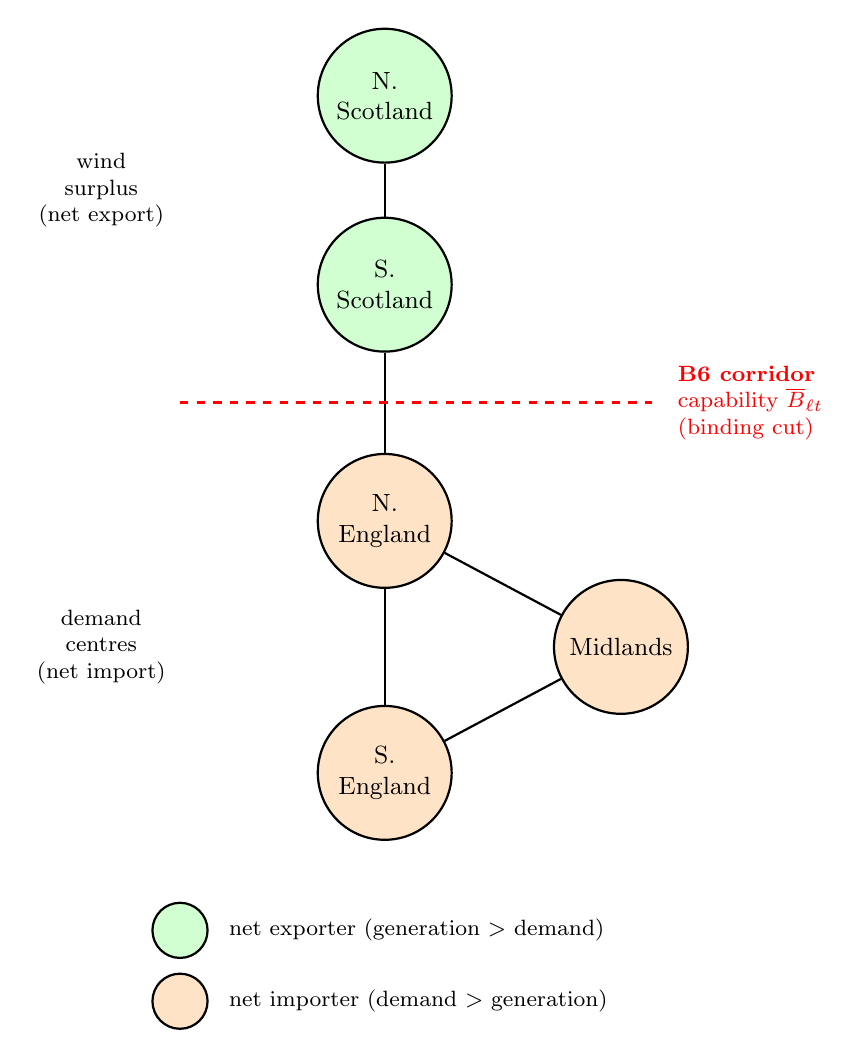
\begin{tikzpicture}[>=Stealth,x=1cm,y=1cm,
  surplus/.style={circle,draw,thick,align=center,font=\small,minimum size=17mm,fill=green!18},
  deficit/.style={circle,draw,thick,align=center,font=\small,minimum size=17mm,fill=orange!22},
  line/.style={thick},
  cut/.style={red,very thick,dashed},
  lbl/.style={font=\footnotesize,align=left}]
% zones, generously spaced along a vertical Scotland->England axis
\node[surplus] (nsc) at (0,8.0)  {N.\\Scotland};
\node[surplus] (ssc) at (0,5.6)  {S.\\Scotland};
\node[deficit] (nen) at (0,2.6)  {N.\\England};
\node[deficit] (mid) at (3.0,1.0){Midlands};
\node[deficit] (sen) at (0,-0.6) {S.\\England};
\draw[line] (nsc)--(ssc);
\draw[line] (ssc)--(nen);
\draw[line] (nen)--(mid);
\draw[line] (nen)--(sen);
\draw[line] (mid)--(sen);
% B6 cut, clearly between S. Scotland and N. England
\draw[cut] (-2.6,4.1) -- (3.4,4.1);
\node[lbl,red,anchor=west] at (3.6,4.1)
   {\textbf{B6 corridor}\\ capability $\overline B_{\ell t}$\\ (binding cut)};
\node[lbl,align=center] at (-3.6,6.8) {wind\\ surplus\\ (net export)};
\node[lbl,align=center] at (-3.6,1.0) {demand\\ centres\\ (net import)};
% legend, placed below the network so it never overlaps the nodes
\begin{scope}[shift={(-2.6,-2.6)}]
  \node[surplus,minimum size=7mm] (lg1) at (0,0) {};
  \node[lbl,anchor=west] at (0.5,0) {net exporter (generation $>$ demand)};
  \node[deficit,minimum size=7mm] (lg2) at (0,-0.9) {};
  \node[lbl,anchor=west] at (0.5,-0.9) {net importer (demand $>$ generation)};
\end{scope}
\end{tikzpicture}
\caption{Stylised GB zonal network. Scottish zones export cheap wind across the
B6 corridor to demand-heavy English zones; when the ETYS capability
$\overline B_{\ell t}$ binds, the network-blind self-schedule is infeasible and
must be redispatched. Node area is indicative only; the geographically resolved
full and B6-reduced networks are shown in Figure~\ref{fig:gbmap}.}
\label{fig:b6map}
\end{figure}

\begin{figure}[t]
\centering
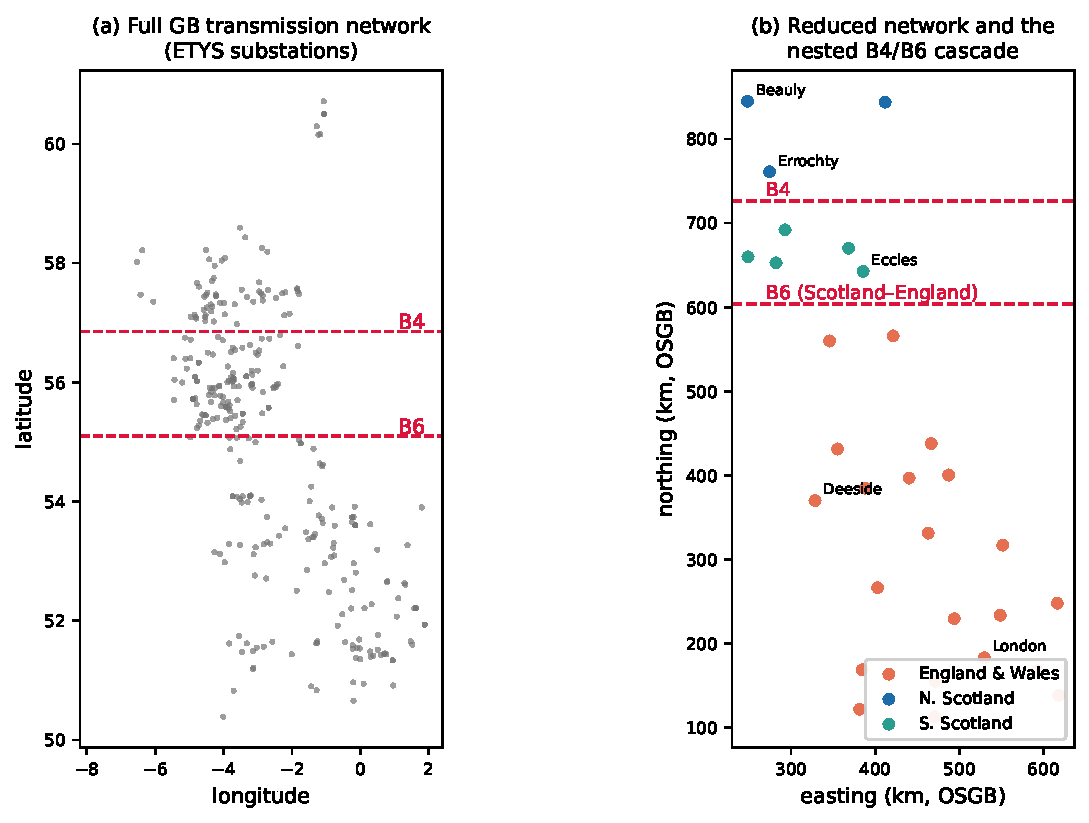
\includegraphics[width=\textwidth]{fig_gbmap}
\caption{The GB transmission network and its reduction, from the open
\textsf{PyPSA-GB} data \citep{pypsagb}. \emph{(a)} the full network: ETYS
substation locations, which trace GB, with the nested B4 and B6 boundaries marked.
\emph{(b)} the reduced 29-bus network (OSGB coordinates), coloured by the three
model zones -- North Scotland, South Scotland and England \& Wales -- separated by
the nested cuts B4 and B6 used by the cascade model of \S\ref{sec:siting}; the
headline B6 study aggregates the two Scottish zones into a single \textsc{sco}
north of B6. Generated by \texttt{make\_gbmap.py}.}
\label{fig:gbmap}
\end{figure}

\begin{example}[The B6 boundary, carried through the paper]
\label{ex:toy}
A single settlement period, two zones \textsc{sco} (Scotland) and \textsc{eng}
(England) joined by the B6 corridor with capability $\overline B=500$\,MW. Demand
is inelastic: $100$\,MW in \textsc{sco}, $900$\,MW in \textsc{eng}. Two
generators: Scottish wind with cost $c_{\mathrm w}=\pounds2$/MWh and capacity
$800$\,MW, and English gas with cost $c_{\mathrm g}=\pounds60$/MWh and ample
capacity. \emph{Stage 1} (network-blind, Problem \eqref{eq:stage1}) clears the cheapest
mix that meets the $1000$\,MW total: wind $800$, gas $200$, setting the national
price $\lambda^{\mathrm{nat}}=\pounds60$/MWh. But this self-schedule sends
$800-100=700$\,MW across B6, exceeding the $500$\,MW capability by $s=200$\,MW, so
it is \emph{infeasible} for the network of Problem \eqref{eq:bench}. \emph{Stage 2}
(redispatch, Problem \eqref{eq:rc}) restores feasibility at least cost by turning wind
\emph{down} $200$\,MW and gas \emph{up} $200$\,MW. At cost-reflective prices the
redispatch cost is $RC=c_{\mathrm g}\cdot 200-c_{\mathrm w}\cdot
200=\pounds11{,}600$, which equals the congestion rent
$R_{\mathrm{cong}}=\pi\, s$ with boundary shadow price
$\pi=c_{\mathrm g}-c_{\mathrm w}=\pounds58$/MWh and relieved overload
$s=200$\,MW (Proposition~\ref{prop:p2}). Because the economy here is convex, the
realised dispatch coincides with the nodal optimum, no make-whole payment is
needed, and the entire cost of national pricing is this $\pounds11{,}600$ of
congestion rent -- collected as merchandising surplus under nodal pricing, but
paid out to generators and socialised under national pricing. Adding a strategic
turn-up markup $\mu$ on the gas offer raises $RC$ by $M=\mu\,c_{\mathrm g}\cdot
200$ (e.g.\ $+\pounds3{,}600$ at $\mu=0.30$); replacing the convex wind unit with
a committable gas unit makes Stage~1 commit blind to the network and opens the
welfare gap of Proposition~\ref{prop:p1}(b). These are exactly the
\texttt{synthetic\_b6} and \texttt{synthetic\_b6\_nonconvex} instances solved by
\texttt{gb\_two\_stage\_skeleton.py} in the repository.
\end{example}

\subsection{The nodal benchmark}
\label{sec:bench}

The network-feasible efficient dispatch maximises welfare subject to zonal
balance, corridor limits and the generators' technical sets:
\begin{align}
\max_{x,y,u,d,f}\;& \sum_{i,t} v_{it}x_{it}-\sum_{j,t}\big(c_{jt}y_{jt}+h_{jt}u_{jt}\big)
\label{eq:bench}\\
\text{s.t.}\;& p_{nt}=\textstyle\sum_{\ell} A_{n\ell}f_{\ell t}
   && \forall n,t\quad(\lambda_{nt}) \notag\\
& -\overline B_{\ell t}\le f_{\ell t}\le \overline B_{\ell t}
   && \forall \ell,t\quad(\pi_{\ell t}) \notag\\
& (y,u,d)\in\mathcal T_j,\;\; 0\le x_{it}\le\overline D_{it},\;\; u_{jt}\in\{0,1\}.
   && \notag
\end{align}
Its optimum is $(x^\ast,y^\ast,u^\ast)$ with welfare $W^\ast$. With the binary
commitment variables $u_{jt}\in\{0,1\}$ present, \eqref{eq:bench} is a
mixed-integer program and the parenthetical multipliers $\lambda_{nt},\pi_{\ell
t}$ are \emph{not} the duals of Problem \eqref{eq:bench} itself -- a nonconvex program has
no exact dual prices. As is standard in nonconvex electricity pricing
\citep{oneill2005, gribik2007, liberopoulos2016}, the prices are defined on a
convex restriction or relaxation: fix the integers at the optimal commitment
$u=u^\ast$ and take the duals of the resulting linear program (integer-programming
pricing), or price on the convex-hull relaxation where  $u_{jt}\in [0,1]$ instead of $u_{jt}\in\{0,1\}$. We adopt this convention throughout: in
the proofs and in the decomposition of Proposition~\ref{prop:p2}, $\lambda_{nt}$
and $\pi_{\ell t}\ge0$ denote the linear-program multipliers of this convex
restriction, the per-zone locational prices and corridor shadow prices
respectively. The gap between the mixed-integer optimum and its convex-hull
relaxation is itself a nonconvexity term, which we report separately rather than
fold into the congestion rent (Remark~\ref{rem:nonconvex}). This is the nodal benchmark, on
top of which we compute the make-whole-minimising PE-A prices of
\citet{bichler2022} and their total $\mathrm{MWP}^{\mathrm{PEA}}$.

\subsection{Stage 1: network-blind national clearing}
\label{sec:stage1}

GB clears energy without the network, collapsing the zonal balances of
Problem \eqref{eq:bench} into a single per-period system balance, and dropping the
corridors and their flows, gives
\begin{align}
\tilde W=\max_{x,y,u,d}\;& \sum_{i,t} v_{it}x_{it}-\sum_{j,t}\big(c_{jt}y_{jt}+h_{jt}u_{jt}\big)
\label{eq:stage1}\\
\text{s.t.}\;& \sum_{n} p_{nt}=0
   && \forall t\quad(\lambda^{\mathrm{nat}}_t) \notag\\
& (y,u,d)\in\mathcal T_j,\;\; 0\le x_{it}\le\overline D_{it},\;\; u_{jt}\in\{0,1\}.
   && \notag
\end{align}
Because Problem \eqref{eq:stage1} relaxes Problem \eqref{eq:bench} (the corridor constraints are
removed), $\tilde W\ge W^\ast$. The single dual $\lambda^{\mathrm{nat}}_t$ of the
system balance is the \emph{national price}: one anonymous price per settlement
period, common to all zones. The optimiser $(\tilde x,\tilde y,\tilde u)$ is the
self-schedule, which is generically infeasible for Problem \eqref{eq:bench}: substituting
$\tilde p_{nt}$ into the corridor definition yields flows that violate some
$\overline B_{\ell t}$. Because $\lambda^{\mathrm{nat}}$ comes from a
mixed-integer program, in computation we recover it as the dual of the balance
in the linear program obtained by fixing $u=\tilde u$, this is the integer-programming
pricing approach of \citet{oneill2005}. Operationally this stage is decentralised -- bilateral, day-ahead and intraday trading -- rather than a
central solver; we use Problem \eqref{eq:stage1} as its competitive proxy and,
empirically, replace $\tilde y$ by the observed self-schedule (\S\ref{sec:corr}).

\subsection{Stage 2: redispatch in the Balancing Mechanism}
\label{sec:stage2}

To make the self-schedule deliverable, NESO accepts turn-up offers (price
$o_{jt}$) and turn-down bids (price $b_{jt}$), moving generation by
$\Delta y_{jt}=y_{jt}-\tilde y_{jt}$. It chooses the network-feasible dispatch of least
redispatch cost:
\begin{align}
RC(o,b)=\min_{x,y,u,d,f}\;& \sum_{j,t}\Big[o_{jt}(y_{jt}-\tilde y_{jt})^{+}
   - b_{jt}(y_{jt}-\tilde y_{jt})^{-}\Big]
\label{eq:rc}\\
\text{s.t.}\;& p_{nt}=\textstyle\sum_{\ell} A_{n\ell}f_{\ell t}
   && \forall n,t\quad(\lambda_{nt})\notag\\
& -\overline B_{\ell t}\le f_{\ell t}\le \overline B_{\ell t}
   && \forall \ell,t\quad(\pi_{\ell t})\notag\\
& (y,u,d)\in\mathcal T_j,\;\; 0\le x_{it}\le\overline D_{it},\;\; u=\tilde u,
   && \notag
\end{align}
 with $(z)^{+}=\max(z,0)$ and $(z)^{-}=\max(-z,0)$. The redispatch multipliers
$\lambda_{nt},\pi_{\ell t}$ carry the same symbols as the nodal benchmark's in
\eqref{eq:bench} by design: with cost-reflective bids ($o=b=c$),
Proposition~\ref{prop:p1} shows the redispatch reproduces the benchmark dispatch,
so at the optimum the two programs' duals coincide -- both are the
convex-restriction multipliers fixed once in \S\ref{sec:bench}.

Three important remarks
\begin{itemize} 
\item[(i)]\emph{Commitment.} Problem~\eqref{eq:rc} holds
self-commitment fixed at $\tilde u$ (the ``tight-BM'' case): the redispatch may
move \emph{committed} units up and down but may not switch units on or off. The
alternative, in which the balancing stage is allowed to start additional units by
paying their start-up and no-load costs, relaxes the last constraint to
$u_{jt}\ge\tilde u_{jt}$ and is what we call \emph{recommitment}. The two are
exposed as a switch in the solver (\texttt{commitment\_policy}), and we show in
Remark~\ref{rem:recommit} below (after Proposition~\ref{prop:p1}) that the choice
between them moves the inefficiency between a welfare loss and an out-of-market
side payment rather than eliminating it; the tight-BM case is the one that makes
Proposition~\ref{prop:p1}(b) sharpest.

\item[(ii)]\emph{ Strategic
markup.} Cost-reflective redispatch sets $o=b=c$; strategic conduct is captured
by a markup $o_{jt}=c_{jt}(1+\mu_{jt})$, $\mu_{jt}\ge 0$, which we \emph{estimate}
from the data (\S\ref{sec:comp}) -- finding it indistinguishable from zero at B6 --
rather than assume, and whose effect we trace as a counterfactual in
\S\ref{sec:sensitivity}.

\item[(iii)]\emph{Curtailment of subsidised wind.} A
support-backed wind unit requires compensation to reduce output, so its
turn-down bid is negative, $b_{jt}<0$; the term $-b_{jt}(\Delta y_{jt})^{-}$ then
contributes a positive cost, which is precisely the curtailment-payment channel
that dominates GB constraint costs. Price-sensitive demand enters symmetrically
through buyer-side acceptances valued at $v$. The realised physical welfare is
$W^{\mathrm{BM}}=W(x^{\mathrm{BM}},y^{\mathrm{BM}},u^{\mathrm{BM}})$, and total
consumer cost is the national energy payment at $\lambda^{\mathrm{nat}}$ plus the
socialised redispatch cost $RC$, recovered from demand through the
Balancing Services Use of System (BSUoS) charge rather than attributed to
identified units.

\end{itemize}

\subsection{From data to model: the settlement correspondence}
\label{sec:corr}

The two stages are not a stylisation imposed on GB, they are its settlement
architecture, and every object in the model is a named, publicly reported
settlement record (Figure~\ref{fig:twostage}), each published by Elexon through
the Balancing Mechanism Reporting Service \citep{elexonbmrs}. Concretely:
\begin{itemize}
\item[--] The Stage-1 self-schedule $\tilde y$ is the \emph{Final Physical
Notification} (FPN): the half-hourly MW profile each Balancing Mechanism Unit
declares at gate closure, one hour ahead of real time. This is the realised,
network-blind self-dispatch.
\item[--] The Stage-2 prices $(o,b)$ are the \emph{Bid--Offer Data} (BOD): the
price--volume ladders each unit submits, an \emph{offer} price to turn up and a
\emph{bid} price to turn down (the latter negative for support-backed wind that
must be paid to curtail).
\item[--] The accepted redispatch $\Delta y$ is read from the \emph{Bid--Offer
Acceptance Level Flagged} dataset (BOALF), which records each acceptance as a
new instructed MW level. Subtracting the FPN gives the accepted volume. Each
acceptance carries a \emph{system (SO) flag}; the SO-flagged acceptances are
those NESO takes for system -- i.e.\ transmission-constraint -- reasons rather than
for energy balancing, and are exactly the redispatch $\Delta y$ of our Stage 2.
\end{itemize}
Returning to Example~\ref{ex:toy}: the $800$\,MW Scottish-wind FPN, its negative
turn-down bid in BOD, and the SO-flagged BOALF acceptance that curtails it by
$200$\,MW (with the matching English-gas turn-up) are precisely the records this
correspondence maps onto $\tilde y$, $b$, and $\Delta y$. Consequently the
redispatch cost $RC$ -- and, as shown later, its decomposition in
Proposition~\ref{prop:p2} -- is largely measurable directly from settlement data,
which we exploit both to calibrate the model and to validate its output against
NESO's published constraint cost.

\begin{figure}[t]
\centering
\resizebox{\textwidth}{!}{%
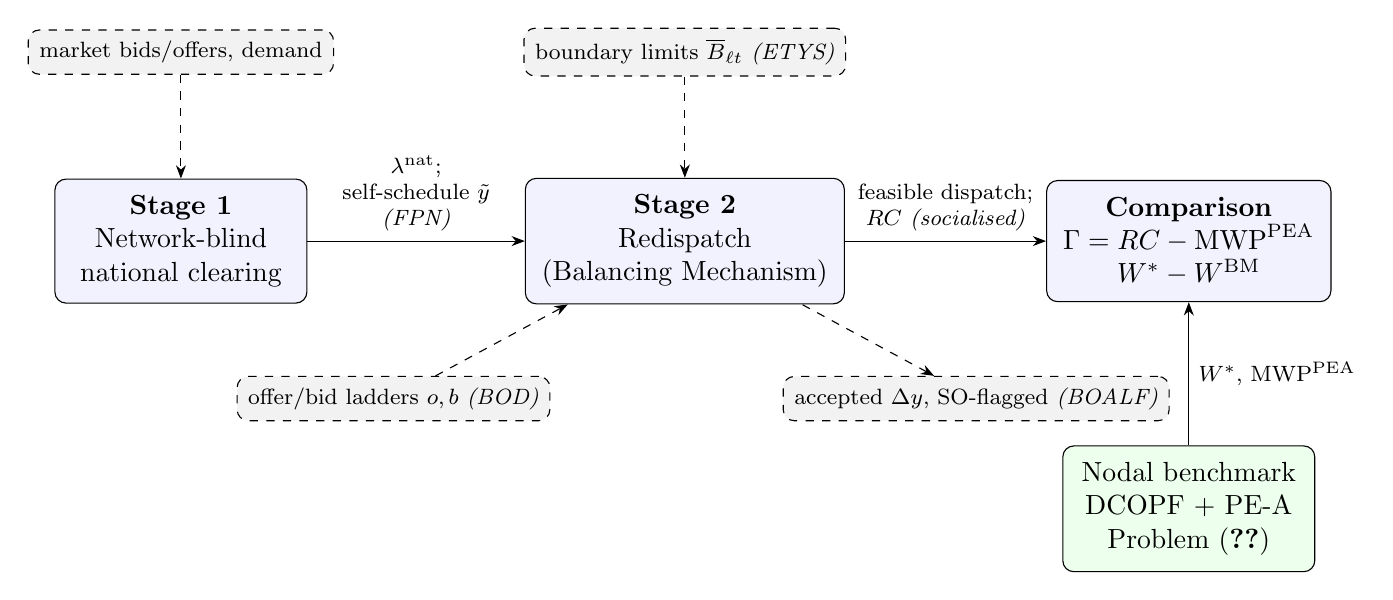
\begin{tikzpicture}[>=Stealth,
  box/.style={draw,rounded corners,align=center,inner sep=6pt,minimum width=32mm,minimum height=15mm,fill=blue!5},
  nb/.style={draw,rounded corners,align=center,inner sep=6pt,minimum width=32mm,minimum height=15mm,fill=green!7},
  db/.style={draw,dashed,rounded corners,align=center,inner sep=4pt,fill=gray!10,font=\footnotesize},
  el/.style={font=\footnotesize,align=center}]
\node[box] (s1) at (0,0)  {\textbf{Stage 1}\\ Network-blind\\ national clearing};
\node[box] (s2) at (6.4,0) {\textbf{Stage 2}\\ Redispatch\\ (Balancing Mechanism)};
\node[box] (g)  at (12.8,0){\textbf{Comparison}\\ $\Gamma=RC-\mathrm{MWP}^{\mathrm{PEA}}$\\ $W^\ast-W^{\mathrm{BM}}$};
\node[nb]  (bn) at (12.8,-3.4){Nodal benchmark\\ DCOPF + PE-A\\ Problem \eqref{eq:bench}};
\draw[->] (s1) -- node[el,above]{$\lambda^{\mathrm{nat}}$;\\ self-schedule $\tilde y$\\ \itshape(FPN)} (s2);
\draw[->] (s2) -- node[el,above]{feasible dispatch;\\ $RC$ \itshape(socialised)} (g);
\draw[->] (bn) -- node[el,right]{$W^\ast$,\ $\mathrm{MWP}^{\mathrm{PEA}}$} (g);
\node[db] (in) at (0,2.4)  {market bids/offers, demand};
\draw[->,dashed] (in) -- (s1);
\node[db] (bd) at (6.4,2.4){boundary limits $\overline B_{\ell t}$ \itshape(ETYS)};
\draw[->,dashed] (bd) -- (s2);
\node[db] (px) at (2.7,-2.0){offer/bid ladders $o,b$ \itshape(BOD)};
\draw[->,dashed] (px) -- (s2);
\node[db] (ba) at (10.1,-2.0){accepted $\Delta y$, SO-flagged \itshape(BOALF)};
\draw[<-,dashed] (ba) -- (s2);
\end{tikzpicture}}
\caption{The two-stage model and its mapping to GB settlement data. A
network-blind national clearing fixes the single price $\lambda^{\mathrm{nat}}$
and the self-schedule $\tilde y$ (observed as FPNs); redispatch then restores
network feasibility using boundary limits (ETYS) and the submitted bid-offer
ladders (BOD), with the accepted, system-flagged volumes recorded in BOALF. The
nodal benchmark supplies $W^\ast$ and the minimised make-whole payments against
which the cost of national pricing $\Gamma$ is measured.}
\label{fig:twostage}
\end{figure}

\subsection{National pricing in the design framework}
\label{sec:framework}

\citet{bichler2022} organise market designs by which of the desiderata they
retain: linear and anonymous prices (LA), individual rationality (IR), budget
balance (BB), and envy-freeness (EF), with side payments restoring IR where
prices alone cannot. National-pricing-with-redispatch is the extreme point of
this framework at which \emph{locational} envy-freeness is relaxed entirely: a
single anonymous price treats a constrained Scottish generator and an English
one identically, and physical feasibility is then bought back through
personalised, pay-as-bid redispatch. Table~\ref{tab:framework} places the three
regimes side by side; the progression from nodal to national trades transparency
of the side payment (attributed make-whole versus socialised redispatch) for
simplicity and a single public price.

\begin{table}[t]
\centering
\caption{Three regimes in the design framework of \citet{bichler2022}. ``Locational
EF'' is envy-freeness across locations; side payments restore IR in all three.}
\label{tab:framework}
\begin{tabular}{lcccl}
\toprule
Regime & Public prices & Locational EF & BB & Side payments \\
\midrule
Nodal (PE-A) & per node & relaxed (2nd order) & near & small, attributed (MWP) \\
Zonal & per zone & partial & no & redispatch (intra-zone) \\
National + redispatch & single & none & no & redispatch, socialised (BSUoS) \\
\bottomrule
\end{tabular}
\end{table}

%  --  --  --  --  --  --  --  --  --  --  --  --  --  --  --  --  --  --  --  --  --  --  %
\section{Theoretical results}
\label{sec:theory}

\paragraph{Preliminaries} Given a feasible solution $(x,y,u)$, its welfare is $W(x,y,u)=v'x-c'y-h'u$. We compare two
feasible sets, both at fixed demand where $x$ is inelastic and price-sensitive
otherwise. The \emph{network-feasible} set $\mathcal F$ collects all
$(x,y,u,d,f)$ satisfying the network-constrained dispatch constraints of the nodal
benchmark \eqref{eq:bench} -- the boundary-transfer
limits $|\!\sum_{\ell\in\beta}f_{\ell t}|\le\overline B_{\beta t}$ together with
the generators' technical sets; its maximiser
is $(x^\ast,y^\ast,u^\ast)$ with value $W^\ast$. The \emph{network-blind} set
$\tilde{\mathcal F}$ drops the flow-definition and boundary-limit constraints; its
maximiser is the self-schedule $(\tilde x,\tilde y,\tilde u)$ with value
$\tilde W$. Dropping constraints enlarges the feasible set, so
$\tilde W\ge W^\ast$. Given the Stage-1 quantities and the offer/bid prices
$o,b$, the redispatch cost $RC(o,b)$ and the realised dispatch
$W^{\mathrm{BM}}$ are those of \eqref{eq:rc}. We state each result with its
economic interpretation here and delegate all  the formal proofs to \ref{app:proofs}.

\begin{proposition}[Nonconvexity is the sole source of inefficiency]
\label{prop:p1}
Assume cost-reflective redispatch, $o=b=c$.
\begin{itemize}
\item[\emph{(i)}] If the economy is convex (no-load costs $h=0$, the commitment
binaries relaxed,  and output is continuously divisible), then
$W^{\mathrm{BM}}=W^\ast$: national-pricing-with-redispatch is welfare-equivalent
to nodal pricing.
\item[\emph{(ii)}] If commitment $u$ is fixed at $\tilde u$, then $W^{\mathrm{BM}}\le W^\ast$, and
$W^\ast-W^{\mathrm{BM}}=0$ only if $\tilde u= u^\ast$.
\end{itemize}
\end{proposition}

The economic reading is that national-pricing-with-redispatch is not
intrinsically inefficient; in a convex world it reproduces the nodal optimum
exactly, because cost-reflective redispatch merely re-solves the dispatch problem
subject to the network. Any realised welfare loss is therefore  purely driven by
nonconvexities: because Stage~1 is blind to the network, it may commit the
wrong set of units (switch on a generator the network cannot accommodate, or
leave off one it needs), and with commitment frozen at $\tilde u$ the redispatch
stage can re-dispatch within that committed fleet but cannot start or stop units
to repair the commitment error.

Part~(i) on its own restates a property that is well understood in the
locational-pricing literature: with cost-reflective bids a redispatch that
restores network feasibility merely re-solves the dispatch program, so in a convex
economy it lands on the nodal optimum. We state it not for novelty but because it
does two things for the rest of the paper. First, it pins every unit of realised
welfare loss to commitment nonconvexity (part~(ii)): in the convex world there is
none, so whatever loss is observed must come from the fixed commitment $\tilde u$.
Second, it tells us how to read the decomposition of Proposition~\ref{prop:p2}:
because the convex benchmark carries \emph{no} efficiency loss, the congestion-rent
term $R_{\mathrm{cong}}$ is a pure \emph{transfer} -- money moved from consumers to
generators -- rather than a resource cost. The contribution is that pairing, and
its measurement on settlement data, not the convex equivalence on its own.

\begin{remark}[The welfare loss is bounded by the BM's commitment freedom]
\label{rem:recommit}
If the BM may re-optimise commitment -- standing self-committed units down where
the network cannot use them, and starting those it needs -- the constraint
$u=\tilde u$ is relaxed and the feasible set expands toward $\mathcal F$, so the
welfare loss $W^\ast-W^{\mathrm{BM}}$ of Proposition~\ref{prop:p1}(b) shrinks,
reaching zero under full recommitment. However, the recovery is not free: it is achieved
through out-of-market commitment actions (start-up/no-load payments, or standing
units down), settled outside the energy price rather than through it. The
realised loss therefore lies between zero (full recommitment) and the tight-BM
value, with the position governed by how much recommitment the BM performs (the
\texttt{commitment\_policy} switch in the experiments); the tight-BM case
($u=\tilde u$) is the conservative upper bound and the one for which
Proposition~\ref{prop:p1}(b) is sharpest. Either way the inefficiency does not
vanish -- it is relocated from a visible welfare loss to the out-of-market
commitment layer.
\end{remark}

We now decompose the visible cost. Write $\Gamma=RC-\mathrm{MWP}^{\mathrm{PEA}}$
for the gap between the socialised redispatch cost under national pricing and the
minimised make-whole payments $\mathrm{MWP}^{\mathrm{PEA}}$ that nodal PE-A pricing
\citep{bichler2022} would instead incur. As in the nodal benchmark
(\S\ref{sec:bench}), the prices $\pi_{\beta t}\ge0$ below are the boundary-limit
multipliers of the convex (LP/convex-hull) restriction of the dispatch.

\begin{proposition}[Side-payment decomposition]
\label{prop:p2}
Let $y^*$ be the solution for Problem \ref{eq:bench}, and $\tilde y$ the self-schedule for Problem \ref{eq:stage1}. Then with cost-reflective prices augmented by a turn-up markup
$o_{jt}=c_{jt}(1+\mu_{jt})$, $\mu_{jt}\ge0$ we have the following:
\begin{itemize}
\item[\emph{(i)}] \emph{(Non-negativity)} $RC=c'y^\ast-c'\tilde y\ge0$, with
equality iff the self-schedule is network-feasible.
\item[\emph{(ii)}] \emph{(Decomposition)} $RC=R_{\mathrm{cong}}+M$, where the
congestion rent $R_{\mathrm{cong}}=\sum_{\beta,t}\pi_{\beta t}s_{\beta t}$ is the
boundary shadow price times the relieved overload $s_{\beta t}$, and the strategic
markup $M=\sum_{j,t}\mu_{jt}c_{jt}(\Delta y_{jt})^{+}$ is the surcharge on
accepted turn-ups.
\end{itemize}
\end{proposition}

\begin{remark}[The side-payment gap]
\label{rem:gap}
The cost of national pricing relative to nodal pricing is the gap
$\Gamma=RC-\mathrm{MWP}^{\mathrm{PEA}}
=R_{\mathrm{cong}}+M-\mathrm{MWP}^{\mathrm{PEA}}$ (from~(ii)), which is
non-negative whenever $\mathrm{MWP}^{\mathrm{PEA}}\le R_{\mathrm{cong}}+M$. This
condition is mild: \citet{bichler2022} report that PE-A make-whole payments are
negligible in their experiments (the very feature that makes PE-A attractive), so
the right-hand side ($R_{\mathrm{cong}}+M$), which contains the full congestion rent, dominates the left ($\mathrm{MWP}^{\mathrm{PEA}}$)
whenever a boundary binds. The economic content is that the congestion rent nodal
pricing would \emph{collect} as merchandising surplus (and could rebate to
consumers) is, under national pricing, instead \emph{paid out} as redispatch and
socialised; to first order $\Gamma\approx R_{\mathrm{cong}}+M$, so on this margin
national pricing is never cheaper than nodal. The non-negativity is a
binding-boundary statement: where no boundary binds, $RC=R_{\mathrm{cong}}=M=0$ and
$\Gamma=-\mathrm{MWP}^{\mathrm{PEA}}\le0$ -- national pricing is then (weakly)
cheaper, precisely because it avoids the nodal make-whole -- so the cost of
national pricing arises only when the network constrains the self-schedule.
\end{remark}

\begin{remark}[Nonconvex shadow prices]
\label{rem:nonconvex}
With binary commitment the dispatch is a mixed-integer program and exact dual
prices $\pi_{\beta t}$ are not defined, so Proposition~\ref{prop:p2}(ii) is taken
on the LP/convex-hull relaxation of the dispatch (binaries relaxed, or convex-hull
prices in the sense of \citep{gribik2007}) -- the same object NESO-style
locational pricing would use. The gap between the mixed-integer redispatch cost
and its convex-hull relaxation is itself a nonconvexity term; we report it
separately rather than fold it into $R_{\mathrm{cong}}$.
\end{remark}

\subsection{Optimal siting of flexibility across nested boundaries}
\label{sec:siting}

Proposition~\ref{prop:p2} values a \emph{given} placement of flexibility behind a
single cut, which raises the question: given a budget of flexible
capacity -- storage or shiftable demand -- \emph{where} along the network should it
go, and how should it be operated over the day, to reduce the cost of national
pricing the most? With several \emph{nested} GB boundaries (e.g., B4 north of B6) and
storage that moves energy across time, this is a genuine optimisation, which we
now state and solve.

Order the zones along the radial cascade $z=1,\dots,Z$ from the surplus (northern)
end to demand, with nested cuts $\beta=1,\dots,B$; cut $\beta$ separates the first
$z_\beta$ zones from the rest, $z_1<\dots<z_B$ (see Figure \ref{fig:gbmap}), so energy injected at zone $z$ must
cross every cut $\beta$ with $z_\beta\ge z$ to reach demand. A budget $K$ of
flexible storage power is sited, $k_z\ge0$ with $\sum_z k_z\le K$; each store has
energy $k_z D$ (duration $D$) and round-trip efficiency $\eta$, with charge and
discharge bounded by $k_z$ and the usual state-of-charge dynamics across periods
$t$. Writing $C(K)$ for the minimised socialised redispatch (equivalently
generation) cost when the network limits are enforced, and $V(K)=C(0)-C(K)$ for
the value of the budget, the siting-and-operation program is

\begin{align}
C(K)=\min_{k,g,w,F,\sigma,ch,dis}\;&
   \sum_{z,t} c_{z}\,g_{zt}
   \label{eq:fs}\\
\text{s.t.}\;&
   w_{zt}+g_{zt}+dis_{zt}-ch_{zt}-x_{zt}
   =\textstyle\sum_{\beta}A_{z\beta}f_{\beta t}
   && \forall z,t\quad(\lambda_{zt})\notag\\
&  -\overline B_{\beta t}\le f_{\beta t}\le\overline B_{\beta t}
   && \forall \beta,t\quad(\pi_{\beta t})\notag\\
&  \sigma_{zt}=\sigma_{z,t-1}+\sqrt{\eta}\,ch_{zt}-dis_{zt}/\sqrt{\eta}
   && \forall z,t\notag\\
&  ch_{zt}\le k_{z},\;\; dis_{zt}\le k_{z},\;\; \sigma_{zt}\le k_{z}D
   && \forall z,t\quad(\rho_{zt})\notag\\
&  \textstyle\sum_{z}k_{z}\le K,\quad k_z\ge0,\;\;
   0\le w_{zt}\le\overline W_{zt},\;\; g_{zt}\ge0.
   && (\mu)\notag
\end{align}
Here $g_{zt}$ is dispatchable (replacement) generation at
cost $c_{z}$, $w_{zt}\le\overline W_{zt}$ the used wind, $x_{zt}$ the inelastic
demand, $f_{\beta t}$ the flow on cut $\beta$ (incidence $A_{z\beta}$), and
$(\sigma_{zt},ch_{zt},dis_{zt})$ the state of charge, charge and discharge of a
store in zone $z$, all capped by the sited power $k_{z}$ (energy $k_zD$,
round-trip $\eta$). The parenthesised symbols are the constraint duals:
$\lambda_{zt}$ (zonal balance), $\pi_{\beta t}\ge0$ (the cut limits -- the
congestion prices of Proposition~\ref{prop:p2}), $\rho_{zt}\ge0$ (the store's
power/energy caps) and $\mu\ge0$ (the siting budget). Write
$\lambda_z:=\partial V/\partial k_z\ge0$ for the per-MW marginal value of capacity
in $z$; by LP sensitivity it is the aggregate shadow value of zone $z$'s capacity
caps. Problem~\eqref{eq:fs} is solved by \texttt{flex\_siting.py}.



\begin{proposition}[Marginal value and water-filling of flexibility]
\label{prop:p3}
At an optimum of \eqref{eq:fs}:
\begin{itemize}
\item[\emph{(i)}] the marginal value $\lambda_z=\partial V/\partial k_z$ equals the
day-value a store in $z$ extracts by relieving the cuts on its path to demand;
by LP duality it is the optimal arbitrage of the shadow prices $\pi_{\beta t}$ of
those binding cuts, $\lambda_z\ge0$.
\item[\emph{(ii)}]\emph{(Cascade monotonicity.)} Because the cuts are nested, a store
further upstream relieves a superset of the cuts a downstream store does, so
$\lambda_z$ is non-decreasing up the cascade.
\item[\emph{(iii)}] \emph{(Water-filling.)} The budget KKT condition is
$\lambda_z\le\mu$ with equality where $k_z>0$: the optimal siting fills the
highest-marginal-value (most upstream binding) zone first and moves down the
cascade, an interior split equalising marginal values across the zones used.
The single-cut, single-period case recovers the flexibility-equivalence of
\S\ref{sec:discussion}, $\lambda=\pi_\beta$.
\end{itemize}
\end{proposition}

%  --  --  --  --  --  --  --  --  --  --  --  --  --  --  --  --  --  --  --  --  --  --  %
\section{Computational design}
\label{sec:comp}

\paragraph{Models} The computation mirrors the model's structure. Because GB
national pricing is not one optimisation but two solved in sequence -- a
network-blind clearing followed by a redispatch that takes the clearing's output
as fixed data -- we implement the three programs of \S\ref{sec:model} separately:
\begin{enumerate}
\item the network-blind national clearing of Stage~1 Problem \eqref{eq:stage1}, which
determines the self-schedule $\tilde y$ and the national price;
\item the cost-minimising redispatch of Stage~2 Problem \eqref{eq:rc}, with two switches -- %
cost-reflective ($o=b=c$) versus marked-up offers, and commitment held fixed
(tight BM) versus allowed to recommit;
\item the nodal PE-A make-whole minimisation of \citet{bichler2022}, adapted to
the boundary-transfer network, which supplies the benchmark
$\mathrm{MWP}^{\mathrm{PEA}}$.
\end{enumerate}
All three are mixed-integer/linear programs over the same boundary-transfer
network, and from the Stage-2 boundary duals we read off the decomposition
$RC=R_{\mathrm{cong}}+M$ of Proposition~\ref{prop:p2}.

\paragraph{Test systems} We use two test systems of increasing data realism, so
that the mechanism can first be checked against known costs and then measured on
real data. The \emph{first} (controlled) setting is a small \emph{purpose-built}
two-zone unit-commitment instance with known costs
(\texttt{synthetic\_b6} and \texttt{synthetic\_b6\_nonconvex}): a convex
version that isolates the congestion rent and a nonconvex version -- committable
generators with no-load and minimum-load on both sides of B6 -- in which the
network-blind clearing commits the wrong units, so the comparative statics of
Propositions~\ref{prop:p1}--\ref{prop:p2} can be read off against ground truth
(\S\ref{sec:nonconvex}).  The \emph{second} (empirical) setting, which supplies external
validity, is the reduced GB B6 model of
\S\ref{sec:comp}, with boundary capabilities from ETYS (and the observed,
outage-adjusted SCOTEX limit), generation anchored to FUELHH and demand to the
national outturn, and Balancing-Mechanism market data from Elexon.

\paragraph{The settlement--model correspondence} The two stages map exactly
onto observable GB settlement objects: the Stage-1 self-schedule is the Final
Physical Notification (FPN) at gate closure; the Stage-2 redispatch is the set of
bid-offer acceptances carrying the system (SO) flag -- the flag NESO attaches to
an acceptance taken to manage a transmission constraint, as distinct from the
unflagged acceptances used to balance national energy supply and demand -- priced
at the submitted Bid-Offer
Data ladders. The decomposition of Proposition~\ref{prop:p2} is therefore
largely observable.

\paragraph{Calibration, identification and validation} Generators' no-load and
start-up costs are not public; we assign them by technology archetype (e.g., wind, gas) and
calibrate them so that the model reproduces NESO's published aggregate
transmission-constraint cost for the day (the figure NESO reports in its
Balancing Costs publications, $\approx\pounds1.9$bn for 2024/25 at the annual
level), reporting Proposition~\ref{prop:p1}'s welfare loss in bands
rather than as a point estimate. The strategic markup $\mu$ is \emph{estimated}
from the data rather than assumed, by a regression-discontinuity design that
compares the price of system-flagged turn-up acceptances in periods when B6 binds
against periods when it does not. The clean specification (\texttt{estimate\_%
markup\_pooled}) is \emph{within-unit-day}: for a unit turned up in both a binding
and a non-binding period of the same day, we measure the proportional change in
its \emph{own} turn-up offer, so unit and day fixed effects net out the unit's
marginal cost and the day's wholesale level -- exactly the confounders that defeat
a naive offer-versus-wholesale comparison (which is badly upward-biased because
binding periods are low-wholesale overnight/high-wind hours). Pooled over the
sampled days (83 unit-day pairs in which a unit appears on both sides of the
threshold), the estimate is essentially zero: $\hat\mu=0.00$ (s.e.\ $0.007$;
$95\%$ CI $[-0.01,0.02]$), against a spurious $+3.4$ from the naive cross-unit
premium-over-wholesale contrast -- the same binding-vs-non-binding comparison
\emph{without} the unit and day fixed effects, computed alongside the headline by
the same routine (\texttt{estimate\_markup\_pooled}) and reported here only to show
the bias the within-unit-day design removes.
Identification rests on the demanding subsample of unit-days for which the same
unit is accepted in both a binding and a non-binding period, so the count is
modest; but the tightness of the interval shows this is a precisely estimated zero
rather than an underpowered null -- it rules out any boundary markup above about
two percent of the wholesale price, far below the $\sim$30\% replacement-gas
premium documented in \S\ref{sec:intro} that motivates the markup channel.
Units do not raise their turn-up offers when B6 binds: the visible cost is
congestion rent, not a strategic markup -- consistent with the inc-dec literature's
reading that redispatch cost reflects market \emph{design} rather than market
power \citep{hirthschlecht2019}. We therefore take the cost-reflective case
($\mu=0$) as the data-supported headline and treat a positive markup as a
counterfactual (the $\mu$-sweep of \S\ref{sec:sensitivity}).

We reconcile a bottom-up redispatch cost computed directly from SO-flagged
acceptances -- each instructed level held over its half-hour settlement period and
priced at the submitted Bid-Offer Data, decomposed into Scottish-wind curtailment
and replacement turn-up -- against NESO's published constraint cost for the same
day. Two points of scope matter. The bottom-up figure is the cost of
\emph{Balancing Mechanism} bid-offer acceptances, which is the dominant component
of, but smaller than, NESO's published \emph{system} constraint cost: the latter
additionally includes constraint-management actions taken outside the BM
(constraint trades, interconnector actions and other balancing services) that
are not recorded in the BOALF dataset. We therefore validate that the BM
bid-offer cost is a large, plausible share of -- without exceeding -- the published
total (empirically $\approx 79\%$ on the selected day), rather than demanding
equality, and quote the headline only when this holds.

%  --  --  --  --  --  --  --  --  --  --  --  --  --  --  --  --  --  --  --  --  --  --  %
\section{Numerical and empirical results}
\label{sec:results}

We report the two settings in turn: a controlled nonconvex instance that exhibits
the welfare-loss result of Proposition~\ref{prop:p1} against known costs
(\S\ref{sec:nonconvex}), then the GB B6 boundary (\S\ref{sec:b6day} onward).

\subsection{A controlled nonconvex instance (Proposition 1(b))}
\label{sec:nonconvex}

In the GB aggregate the realised welfare loss is essentially zero
(\S\ref{sec:b6day}), as Proposition~\ref{prop:p1}(a) predicts for a near-convex
economy: the cost of national pricing there is congestion rent, not lost dispatch
efficiency. To exhibit the welfare loss of part~(b) -- the genuinely nonconvex
case -- we use the purpose-built instance of \S\ref{sec:comp} with known costs
(\texttt{synthetic\_b6\_nonconvex}; full walk-through in the code). Demand is
$100$ (\textsc{sco}) $+\,1000$ (\textsc{eng})\,MW across a $500$\,MW B6 cut, with
committable units carrying no-load and minimum-load on both sides.

The network-blind clearing commits a cheap committable Scottish unit
($\tilde u=\{\textsc{sco\_ccgt},\textsc{eng\_base}\}$; the costs are illustrative,
not technology-calibrated), but the network optimum
serves the north with wind alone and leaves that unit off
($u^\ast=\{\textsc{eng\_base}\}$): $\tilde u\neq u^\ast$. Under the tight BM the
mis-committed unit cannot be stood down -- it is stranded at its minimum stable
load behind B6 -- so $W^{\mathrm{BM}}<W^\ast$. Table~\ref{tab:nonconvex} reports
the result: a welfare loss of $\pounds4{,}800$, decomposing into a $\pounds2{,}800$
minimum-load component (the stranded unit displacing cheaper wind) and a
$\pounds2{,}000$ no-load component, and growing linearly with the no-load cost.
The loss is exactly zero in the convex instance, confirming
Proposition~\ref{prop:p1}(a), and is recovered in full by recommitment, as in
Remark~\ref{rem:recommit}.

\begin{table}[t]
\centering
\caption{Proposition~\ref{prop:p1} on controlled instances with known costs
(\texttt{nonconvex\_experiment.py}). The welfare loss is a purely driven by
commitment-nonconvexity: zero when convex, growing with the no-load cost,
recovered by recommitment.}
\label{tab:nonconvex}
\begin{tabular}{lr}
\toprule
Instance / regime & Welfare loss $W^\ast-W^{\mathrm{BM}}$ (\pounds)\\
\midrule
Convex (\texttt{synthetic\_b6}) & $0$\\
\midrule
Nonconvex, tight BM & $4{,}800$\\
\quad of which minimum-load component (no-load $\leftarrow 0$) & $2{,}800$\\
\quad of which no-load component & $2{,}000$\\
Nonconvex, recommitment & $0$\\
\midrule
\multicolumn{2}{l}{\emph{Comparative static: tight-BM loss vs no-load scale $\theta$}}\\
$\theta=0$ \;\,(min-load only) & $2{,}800$\\
$\theta=0.5$ & $3{,}800$\\
$\theta=1.0$ \;(baseline) & $4{,}800$\\
\bottomrule
\end{tabular}
\end{table}

\subsection{The GB B6 boundary: a peak-curtailment day}
\label{sec:b6day}

We select the peak-curtailment day in winter 2024/25 by ranking candidate days
on total system-flagged Scottish-wind turn-down volume, then solve every
settlement period and aggregate. Table~\ref{tab:results} reports the daily
totals; the reconciliation against the published constraint cost is reported
alongside.

\begin{table}[t]
\centering
\caption{Modelled cost of national pricing on the B6 boundary, 8 December 2024
(daily totals, \pounds; FUELHH/demand-anchored two-zone instance, central
calibration; \texttt{run\_paper.py}). The cost-reflective column is the
data-supported case ($\hat\mu\approx0$; \S\ref{sec:comp}); the second is a
$\mu=0.30$ \emph{counterfactual} (set to the $\approx30\%$ replacement-gas premium
over wholesale documented in \S\ref{sec:intro}). The rows read top-to-bottom as the
Proposition~\ref{prop:p2} decomposition. The data validation is in the text.}
\label{tab:results}
\begin{tabular}{lrr}
\toprule
Quantity & Cost-reflective & Markup counterfactual\\
 & $(o=b=c)$ & $(\mu=0.30)$\\
\midrule
Congestion rent $R_{\mathrm{cong}}$              & $2{,}883{,}000$ & $2{,}883{,}000$\\
\quad${}+{}$ strategic markup $M$                & $0$             & $368{,}000$\\
\cmidrule(l){2-3}
\quad${}={}$ redispatch cost $RC$                & $2{,}883{,}000$ & $3{,}251{,}000$\\
\quad${}-{}$ nodal make-whole $\mathrm{MWP}^{\mathrm{PEA}}$ & $0$  & $0$\\
\cmidrule(l){2-3}
\quad${}={}$ gap $\Gamma=RC-\mathrm{MWP}^{\mathrm{PEA}}$                        & $2{,}883{,}000$ & $3{,}251{,}000$\\
\addlinespace
Welfare loss $W^\ast-W^{\mathrm{BM}}$ (Prop.~\ref{prop:p1}) & $0$ & $0$\\
\bottomrule
\end{tabular}
\end{table}


The validation panel confirms the data pipeline: the bottom-up cost of
SO-flagged BM bid-offer acceptances -- every flagged acceptance on the day priced
at its submitted Bid-Offer Data and summed over the 48 periods
(\texttt{redispatch\_cost\_detailed}), $\pounds8.76$m -- is $79\%$ of NESO's
published system constraint cost ($\pounds11.1$m), the residual being the non-BM
constraint actions discussed in \S\ref{sec:comp}. This day-level figure is the
reconciliation anchor (it checks that our reading of the settlement data is sound);
it is not the headline, which is the directly-measured annual rent of
\S\ref{sec:annual}. The reconciliation passes, so the modelled figures are quoted. The modelled
quantities are the B6 two-zone reduction under the central calibration; the
welfare loss is zero because the aggregate is convex, so -- exactly as in the
worked Example~\ref{ex:toy}, where $RC=R_{\mathrm{cong}}=\pounds11{,}600$ and
$\mathrm{MWP}^{\mathrm{PEA}}=0$ -- the entire cost of national pricing surfaces as
$\Gamma=R_{\mathrm{cong}}$, here $\approx\pounds2.88$m for the day. The
markup counterfactual ($\mu=0.30$, the \S\ref{sec:intro} replacement-gas premium)
adds $\pounds0.37$m, but the data-driven
markup is $\approx0$ (\S\ref{sec:comp}), so the cost-reflective column is the one
we carry forward.

Consistent with Proposition~\ref{prop:p1}(a), in the aggregated convex
representation the realised welfare loss is zero and the cost of national
pricing surfaces entirely as the congestion rent $R_{\mathrm{cong}}$ (the markup
$M\approx0$ in the data); the data validation closes the loop: reconstructing the
SO-flagged BM constraint cost from settlement records recovers $79\%$ of NESO's
published system constraint cost, the remainder being constraint actions taken
outside the Balancing Mechanism, which confirms that our reading of the
settlement data is sound.

\subsection{From a day to a year: a data-anchored annual cost}
\label{sec:annual}

A single day cannot speak to the magnitude that drives the policy debate -- NESO's
annual constraint cost of $\approx\pounds1.9$bn -- so we scale to a year, but doing
so exposes a calibration question that we resolve with observed boundary data.

\paragraph{Why the structural model is not used for the level} The two-zone
instance of \S\ref{sec:comp} reproduces the \emph{mechanism} of
Proposition~\ref{prop:p2} and is well suited to the comparative statics below,
where only \emph{relative} responses matter. Its absolute level, however, is
sensitive to two stylised inputs -- how much GB wind sits behind B6, and the
boundary capability. Anchoring the capability to NESO's published, outage-adjusted
B6 (SCOTEX) limit, which falls as low as $2.5$\,GW on fault days rather than the
$\approx6$\,GW ETYS headline, swings the modelled annual rent from $\pounds165$m
(fixed limit) to $\pounds754$m (observed fault-day limits, $\pm142$ SE) -- both
below the directly measured $\pounds1.1$bn of the following section. The structural
reduction cannot, with a single Scottish-wind share, simultaneously match the
observed curtailment volume and the days on which it occurs, because the effective
capability varies day-to-day with network faults that a fixed two-zone reduction
does not represent, so it understates the realised cost. We therefore do not quote
the structural model as the level; we measure the level directly.

\paragraph{A realised, settlement-data measure} The relieved overload is
\emph{observed}: it is the volume of system-flagged Scottish-wind turn-down in
BOALF, i.e.\ the curtailment NESO actually instructed to keep B6 within its limit.
Scottish (north-of-B6) units are identified from the BMRS registry by GSP group
together with the zonal transmission loss factor (the latter is essential, as
transmission-connected units carry no GSP group); \ref{app:classif} shows the
annual figure is invariant to the loss-factor cut and cross-checks the selected
units by name.
Pricing each curtailed MWh at the boundary rent -- the wholesale replacement price
south of the cut less the unit's (negative) turn-down bid -- gives the realised B6
congestion rent directly from settlement records, with no zonal-share assumption.
(we use the SCOTEX \emph{limit} but not its \emph{flow} field, which is a
day-ahead \emph{unconstrained} forecast that can exceed B6's physical capacity and
so overstates the realised overload.)

\paragraph{Annualisation} Daily costs are highly skewed (the busiest tenth of
days carries about a third of the annual total), so we estimate the annual total
by \emph{stratified sampling}, using NESO's published daily series as both the
stratifying variable and an independent anchor. We retrieve NESO's daily
\emph{system} constraint cost for all $365$ days of FY 2024/25 (it sums to
$\pounds1{,}903$m), sort the days into five equal-count bins by that cost, draw a
random sample of six days per bin ($30$ days), compute the realised B6 rent for
each, and form the stratified estimator $\widehat{C}=\sum_b N_b\,\bar c_b$ with its
standard error ($N_b$ the days in bin $b$, $\bar c_b$ the sample mean there). This
is \texttt{run\_annual.py}.

Table~\ref{tab:annual} reports the result. The realised B6 congestion rent tracks
the independent NESO daily series almost exactly (day-level correlation $0.97$) and
aggregates to $\pounds1{,}126$m/yr ($\pm\pounds98$m), on $9.55$\,TWh of
Balancing-Mechanism-visible Scottish-wind curtailment -- about $59\%$ of the
system-wide constraint cost. The comparison is like-for-like: both the realised
rent and NESO's published constraint cost are the payment to turn Scottish wind
\emph{down} plus the payment to turn replacement generation \emph{up}, so the
share is a genuine fraction of the same quantity rather than a ratio of
differently-defined costs -- and if anything it is conservative, because we value
the replacement leg at the wholesale index rather than at the (higher) accepted
offer price NESO actually pays. National-pricing redispatch on the single B6
boundary therefore costs of order $\pounds1$bn/yr and is the dominant component of
GB constraint costs.

Two checks support the magnitude. \emph{External corroboration:} our
settlement-derived $9.55$\,TWh (FY 2024/25) is consistent with independently
published curtailment volumes -- the Renewable Energy Foundation, also working from
BMRS settlement records, reports $8.3$\,TWh of GB wind curtailed in calendar 2024,
the great majority Scottish \citep{ref2025}, and FY 2024/25 extends into the
higher-curtailment 2025 period -- so the figure matches the public record rather
than being a partial measure. \emph{B6 attribution:} $97\%$ of the curtailed
volume falls in settlement periods where the real-time
(physical-notification-implied) northward flow exceeds NESO's outage-adjusted
SCOTEX limit, confirming the turn-down relieves the Scotland--England constraint
rather than local intra-Scotland faults (the day-ahead SCOTEX \emph{flow} field is
an unconstrained forecast and under-predicts on exactly the high-wind days, so it
is not used for this test). The $41\%$ residual of the system total reflects other
boundaries, thermal and voltage actions, and non-curtailment constraint costs. The
one component our Balancing-Mechanism measure still omits is curtailment of
\emph{embedded} (distribution-connected) Scottish wind, which settles outside the
Mechanism; including it would raise the figure modestly further, so $\pounds1.1$bn
is, if anything, a mild lower bound on the full B6 cost. A complete
embedded-inclusive figure requires the multi-zone reduced-network build, which is left to
future work.

\begin{table}[t]
\centering
\caption{Annualised cost of national pricing on the B6 boundary, FY 2024/25,
from a 30-day stratified sample (\texttt{run\_annual.py}). The realised rent is
measured directly from settlement data; the NESO figure is the published
\emph{system-wide} annual constraint cost (all boundaries and causes). ``SE'' is
the standard error of the stratified estimator.}
\label{tab:annual}
\begin{tabular}{lr}
\toprule
Quantity & Value\\
\midrule
\multicolumn{2}{l}{\emph{Headline (data-driven)}}\\
Realised B6 congestion rent & $\pounds1{,}126$m/yr $(\pm 98\ \text{SE})$\\
\addlinespace
\multicolumn{2}{l}{\emph{Diagnostics (not components of the rent)}}\\
BM-visible Scottish-wind curtailment & $9.55$\,TWh/yr\\
Correlation of daily rent with NESO series & $0.97$\\
Realised B6 rent as share of system total & $59\%$\\
Curtailment in real-time B6-binding periods & $97\%$\\
\addlinespace
\multicolumn{2}{l}{\emph{For reference}}\\
Published GB wind curtailment, CY2024 \citep{ref2025} & $8.3$\,TWh/yr\\
NESO published \emph{system} constraint cost & $\pounds1{,}903$m/yr\\
\bottomrule
\end{tabular}
\end{table}


\subsection{Scaling and sensitivity}
\label{sec:sensitivity}

Because the policy interest is in how the cost of national pricing moves with the
levers REMA can pull, we sweep each of four levers (B6 capability, Wind penetration, Flexibility behind B6, and Strategic markup) on the same day, holding the
others at their central calibration, with \texttt{sensitivity.py}. Each sweep
re-solves all $48$ periods, Figure~\ref{fig:sens} reports the resulting daily
totals, and the full grids are in \ref{app:sensitivity}.

\begin{figure}[t]
\centering
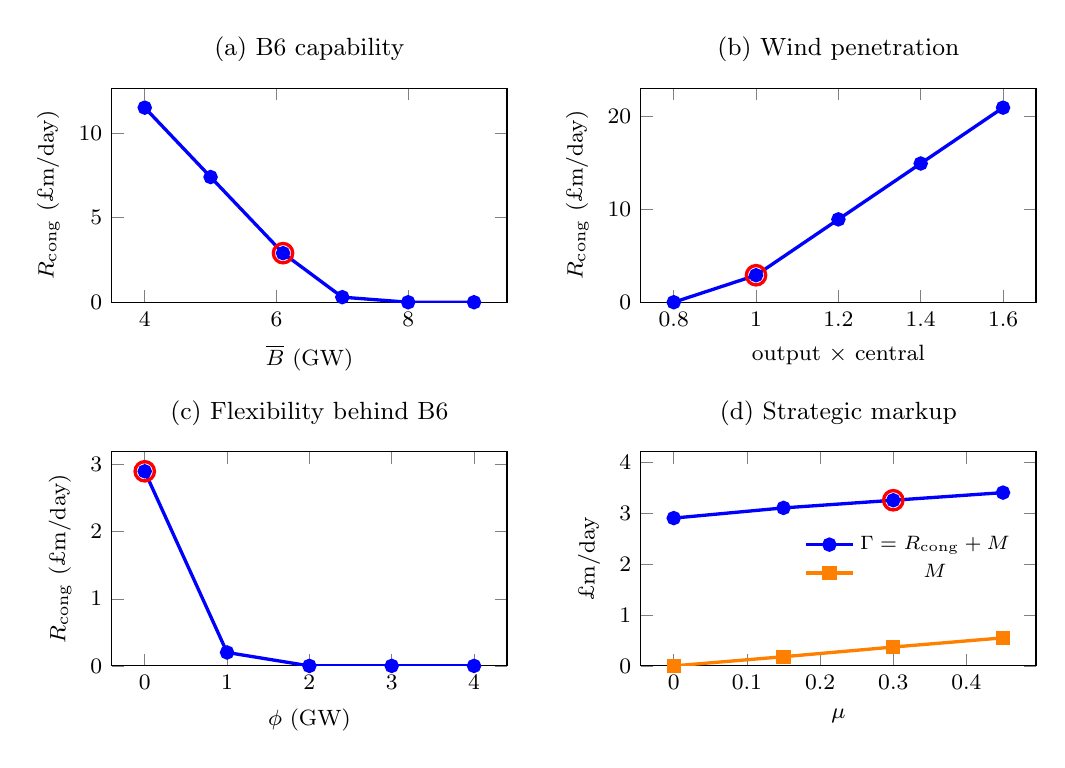
\begin{tikzpicture}
\begin{groupplot}[
  group style={group size=2 by 2, horizontal sep=1.7cm, vertical sep=1.9cm},
  width=6.6cm, height=4.3cm,
  tick label style={font=\footnotesize}, label style={font=\footnotesize},
  title style={font=\small}, ymin=0,
  every axis plot/.append style={very thick}]
% (a) B6 capability
\nextgroupplot[title={(a) B6 capability}, xlabel={$\overline B$ (GW)},
  ylabel={$R_{\mathrm{cong}}$ (\pounds m/day)}]
\addplot[mark=*,blue] coordinates {(4,11.5)(5,7.4)(6.1,2.9)(7,0.3)(8,0)(9,0)};
\addplot[mark=o,red,only marks,mark size=3.5pt] coordinates {(6.1,2.9)};
% (b) Wind penetration
\nextgroupplot[title={(b) Wind penetration}, xlabel={output $\times$ central},
  ylabel={$R_{\mathrm{cong}}$ (\pounds m/day)}]
\addplot[mark=*,blue] coordinates {(0.8,0)(1.0,2.9)(1.2,8.9)(1.4,14.9)(1.6,20.9)};
\addplot[mark=o,red,only marks,mark size=3.5pt] coordinates {(1.0,2.9)};
% (c) Flexibility behind boundary
\nextgroupplot[title={(c) Flexibility behind B6}, xlabel={$\phi$ (GW)},
  ylabel={$R_{\mathrm{cong}}$ (\pounds m/day)}]
\addplot[mark=*,blue] coordinates {(0,2.9)(1,0.2)(2,0)(3,0)(4,0)};
\addplot[mark=o,red,only marks,mark size=3.5pt] coordinates {(0,2.9)};
% (d) Strategic markup
\nextgroupplot[title={(d) Strategic markup}, xlabel={$\mu$},
  ylabel={\pounds m/day}, ymax=4.2,
  legend style={font=\scriptsize,draw=none,at={(0.97,0.5)},anchor=east}]
\addplot[mark=*,blue] coordinates {(0,2.9)(0.15,3.1)(0.30,3.25)(0.45,3.4)};
\addlegendentry{$\Gamma=R_{\mathrm{cong}}+M$}
\addplot[mark=square*,orange] coordinates {(0,0)(0.15,0.18)(0.30,0.37)(0.45,0.55)};
\addlegendentry{$M$}
\addplot[mark=o,red,only marks,mark size=3.5pt] coordinates {(0.30,3.25)};
\end{groupplot}
\end{tikzpicture}

\caption{Comparative statics on the B6 boundary, 8 December 2024 (daily totals).
Each panel sweeps one lever, holding the others at the central calibration (red
ring). Panels (a)--(c) report the congestion rent $R_{\mathrm{cong}}$; panel (d)
the gap $\Gamma=R_{\mathrm{cong}}+M$ and its markup component $M$. Transmission
build-out (a) and behind-boundary flexibility (c) drive the rent to zero;
wind growth (b) raises it near-linearly; the markup (d) is additive. Numeric
grids in \ref{app:sensitivity}; produced by \texttt{sensitivity.py}.}
\label{fig:sens}
\end{figure}

The four statics are exactly the policy levers discussed in \S\ref{sec:discussion}, and each
behaves as the theory predicts.
\begin{itemize}
\item[--] \emph{B6 capability.} Transmission build-out reduces the relieved
overload one-for-one: widening B6 from $6.1$ to $7.0$\,GW cuts $R_{\mathrm{cong}}$
from $\pounds2.9$m to $\pounds0.3$m per day, and at $\approx8$\,GW the
self-schedule is network-feasible and $R_{\mathrm{cong}}=0$, precisely
Proposition~\ref{prop:p2}(i).
\item[--] \emph{Wind penetration (Clean Power 2030).} Above the binding threshold
$R_{\mathrm{cong}}$ rises essentially linearly -- about $\pounds6$m per day for each
$0.2\times$ increment of Scottish wind output -- so the cost of retaining national
pricing scales steeply along the FES trajectory; below $\approx0.9\times$ the
boundary stops binding.
\item[--] \emph{Flexibility behind the boundary.} Relocating flexible demand or
storage north of B6 absorbs the surplus locally: $\approx2$\,GW eliminates
$R_{\mathrm{cong}}$ entirely. This is the flexibility-equivalence result of
\S\ref{sec:discussion} in numbers -- each MW of behind-boundary flexibility is
worth the boundary shadow price in avoided socialised redispatch.
\item[--] \emph{Markup (counterfactual).} The strategic component $M$ is linear in
$\mu$ ($\approx\pounds1.2$m per unit $\mu$) and additive on the congestion rent,
$\Gamma=R_{\mathrm{cong}}+M$; it is the part of the gap that BM-competition
measures, rather than transmission or flexibility, would address. Since the
within-unit-day estimate is $\hat\mu\approx0$ (\S\ref{sec:comp}), panel~(d) is a
counterfactual: at B6 today $M\approx0$ and the gap is essentially
$R_{\mathrm{cong}}$.
\end{itemize}

\subsection{Optimal flexibility siting (Proposition~\ref{prop:p3})}
\label{sec:siting-num}

Following the analysis from the previous section, we now explore the role of flexibility. We solve the
full siting-and-operation program \eqref{eq:fs} on a stylised nested instance with
known costs (\texttt{flex\_siting.py}): a North~Scotland\,$\to$\,South
Scotland\,$\to$\,England chain across the nested cuts B4 and B6, a diurnal wind
profile anti-correlated with the English demand peak, and 4-hour storage of budget
$K$ to be sited in the north and/or south. Both cuts bind, so northern storage
relieves \emph{both} (it captures wind trapped behind B4 and arbitrages B6) while
southern storage relieves \emph{only} B6.

Figure~\ref{fig:siting} reports the value of the budget, $V(K)$, for the optimal
siting and for the two pure placements. Three features confirm
Proposition~\ref{prop:p3}. First, \emph{siting is decisive}: placing the whole
budget in the south captures only $\approx\pounds52$k/day, against
$\approx\pounds480$k for the north and up to $\approx\pounds533$k for the optimum
 -- getting the location wrong forfeits roughly nine-tenths of the value. Second,
the \emph{optimum water-fills the cascade}: it fills the north (higher marginal
value, relieving both cuts) first, then spills into the south once the north's
marginal value has fallen, so the optimal split strictly beats either pure
placement once the budget exceeds the north's useful capacity. Third, the value is
\emph{concave and saturates} ($\approx\pounds0.53$m/day here) once flexibility has
absorbed the binding surplus, the multi-period analogue of $R_{\mathrm{cong}}\to0$
in \S\ref{sec:sensitivity}.

\begin{figure}[t]
\centering
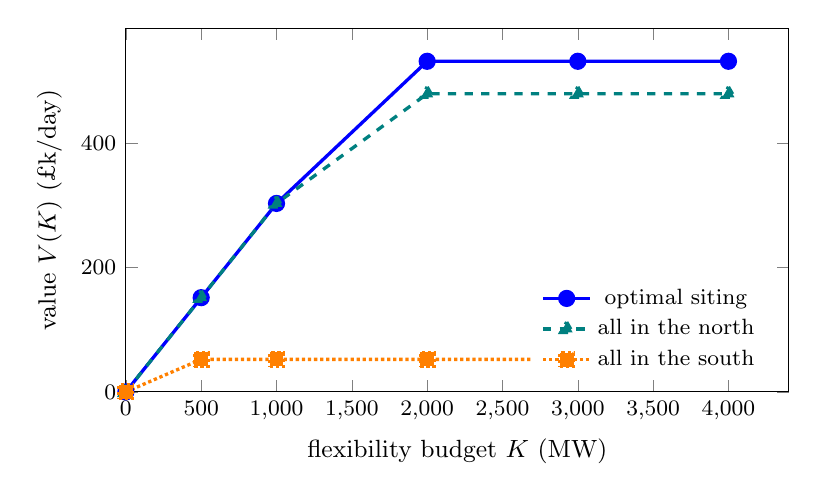
\begin{tikzpicture}
\begin{axis}[width=10cm, height=6.2cm, xlabel={flexibility budget $K$ (MW)},
  ylabel={value $V(K)$ (\pounds k/day)}, xmin=0, ymin=0,
  legend pos=south east, legend style={font=\footnotesize,draw=none},
  tick label style={font=\footnotesize}, label style={font=\small},
  every axis plot/.append style={very thick, mark size=2.5pt}]
\addplot[blue,mark=*] coordinates {(0,0)(500,151.8)(1000,303.6)(2000,532.6)(3000,532.6)(4000,532.6)};
\addlegendentry{optimal siting}
\addplot[teal,mark=triangle*,dashed] coordinates {(0,0)(500,151.8)(1000,303.6)(2000,480.2)(3000,480.2)(4000,480.2)};
\addlegendentry{all in the north}
\addplot[orange,mark=square*,densely dotted] coordinates {(0,0)(500,52.4)(1000,52.4)(2000,52.4)(3000,52.4)(4000,52.4)};
\addlegendentry{all in the south}
\end{axis}
\end{tikzpicture}
\caption{Value of a flexibility budget on the nested B4/B6 cascade (stylised
instance, daily totals; \texttt{flex\_siting.py}). Optimal siting water-fills the
north (relieving both cuts) before the south; placing the budget south of the
binding B4 cut captures almost none of the value; the value is concave and
saturates. This is Proposition~\ref{prop:p3} in numbers.}
\label{fig:siting}
\end{figure}

%  --  --  --  --  --  --  --  --  --  --  --  --  --  --  --  --  --  --  --  --  --  --  %
\section{Discussion and policy implications}
\label{sec:discussion}

The results give a precise reading of REMA's choice. Retaining national pricing
does not, in a near-convex aggregate, sacrifice much dispatch efficiency; its
cost is the congestion rent that a locational price would have internalised,
here paid out as redispatch and socialised through balancing charges, plus a
strategic markup. This reframes the reformed-national-pricing agenda: measures
that reduce the binding congestion (transmission build-out, strategic siting) or
that place flexible demand and storage behind the boundary act directly on
$R_{\mathrm{cong}}$, while measures that improve BM competition act on $M$.

We make the flexibility channel precise. Suppose a quantity $\phi_{\beta t}\ge0$
of flexible resource -- price-sensitive demand, storage, or shiftable load -- sits
north of the binding cut and can absorb surplus locally. Its first-order effect is
to reduce the relieved overload one-for-one, $s_{\beta t}(\phi)=
(s_{\beta t}(0)-\phi_{\beta t})^{+}$, so that, by Proposition~\ref{prop:p2}(ii),
the congestion-rent component falls as
$R_{\mathrm{cong}}(\phi)=\sum_{\beta,t}\pi_{\beta t}\,(s_{\beta t}(0)-
\phi_{\beta t})^{+}$ and reaches its uplift-only minimum once
$\phi_{\beta t}\ge s_{\beta t}(0)$ for all binding $(\beta,t)$, i.e.\ once enough
locational flexibility makes the self-schedule network-feasible. This
\emph{flexibility-equivalence} result -- a given megawatt of behind-the-boundary
flexibility is worth the boundary shadow price $\pi_{\beta t}$ in avoided
socialised redispatch -- formalises the central premise of REMA's reformed
national-pricing model. \emph{Where} that flexibility should sit, when several
boundaries bind, is the optimal-siting problem we solve in
\S\ref{sec:siting}: Proposition~\ref{prop:p3} shows the marginal value of siting
rises up the nested cascade (a megawatt in the far north relieves every cut it
sits behind, not just the nearest), and that the budget should water-fill the
most upstream binding location first. The numerical instance of
\S\ref{sec:siting-num} bears this out starkly -- siting the budget south of the
binding cut forfeits roughly nine-tenths of the value. This turns ``strategic
siting'' from a slogan into a ranked, quantified prescription. The remaining
extension, integrating the siting decision with the strategic markup $M$ and the
full multi-zone reduced network, is left to future work.

%  --  --  --  --  --  --  --  --  --  --  --  --  --  --  --  --  --  --  --  --  --  --  %
\section{Conclusion}
\label{sec:conclusion}

This paper has characterised the cost of national electricity pricing as a
two-stage phenomenon -- a network-blind national clearing followed by a
cost-minimising redispatch -- and located that institution as the extreme,
locational-envy-freeness-relaxing point of the side-payment design framework of
\citet{bichler2022}. The contribution is fivefold. First, a model: we formalise
GB self-dispatch-with-redispatch as the composition of three programs whose
objects coincide exactly with the published settlement records (FPN, BOD,
SO-flagged BOALF), so the theory is measurable rather than merely illustrative.
Second, an efficiency result (Proposition~\ref{prop:p1}): national pricing with
cost-reflective redispatch is welfare-equivalent to nodal pricing in a convex
economy, so any realised welfare loss is a purely driven by commitment-nonconvexity
-- and, under recommitment, even that loss migrates into an out-of-market
side payment rather than vanishing. Third, a decomposition
(Proposition~\ref{prop:p2}): the visible cost splits into a congestion-rent term
that nodal pricing would \emph{collect} as merchandising surplus but national
pricing \emph{pays out} and socialises, plus a strategic redispatch markup, with
a gap to the minimised nodal make-whole payments that is non-negative under an
empirically supported condition. Fourth, a measurement: exploiting the
settlement correspondence and a FUELHH/demand-anchored reduction of the
Scotland--England (B6) boundary, we quantify the cost for a peak-curtailment day
and scale it, by a settlement-data stratified estimator, to a directly measured
annual B6 congestion rent of order $\pounds1.1$bn in FY 2024/25 ($\approx59\%$ of
GB system constraint cost, correlation $0.97$ with the published daily series),
validate the bottom-up Balancing Mechanism cost against NESO's published
constraint cost, and trace how the figure responds to the levers in the reform
debate -- transmission build-out and behind-boundary flexibility both drive the
congestion rent to zero, wind growth raises it steeply, and BM competition acts
only on the markup. Fifth, an optimisation (Proposition~\ref{prop:p3}): we cast
the placement of flexibility across the nested GB boundaries as a
siting-and-operation program and show its marginal value rises up the cascade and
that the budget should water-fill the most upstream binding location first -- a
ranked, quantified version of ``strategic siting'' in which placing flexibility on
the wrong side of a binding cut forfeits almost all of its value.

Two readings follow for policy. The efficiency case against national pricing is,
in a near-convex aggregate, weaker than often asserted: the first-order cost is
not foregone dispatch efficiency but congestion rent that is paid out and
socialised rather than internalised and rebated. And the reformed-national-pricing
agenda has a precise target -- measures that relieve the binding boundary
(transmission, siting, storage and flexible demand behind the cut) act directly on
$R_{\mathrm{cong}}$, while measures that sharpen balancing-market competition act
on $M$ -- though at B6 we find $M$ empirically negligible, so the first-order
target is $R_{\mathrm{cong}}$. Several extensions are natural: a full multi-zone
build on the NESO Reduced Model and Future Energy Scenarios (which would also
capture embedded-wind curtailment settled outside the Balancing Mechanism), and joint
optimisation of flexibility siting with the strategic markup. More broadly, the
framework is not specific to electricity: it applies to any two-stage market that
clears at a uniform price and restores feasibility through a subsequent redispatch.
%  --  --  --  --  --  --  --  --  --  --  --  --  --  --  --  --  --  --  --  --  --  --  %
\section*{Reproducibility}
The optimisation models, including the Proposition~\ref{prop:p2} decomposition
$RC=R_{\mathrm{cong}}+M$ recovered from the boundary LP duals
(\texttt{gb\_two\_stage\_skeleton.py}), the public BMRS Insights client
(\texttt{bmrs\_client.py}), the empirical pipeline wiring PN/BOD/BOALF into the
model, estimating the strategic markup $\mu$ by the within-unit-day
regression discontinuity (\texttt{estimate\_markup\_pooled}) and reconciling the data-derived redispatch cost
against the published NESO constraint cost (\texttt{gb\_empirical\_pipeline.py},
function \texttt{reconcile}), the orchestration that produces
Table~\ref{tab:results} (\texttt{run\_paper.py}), the controlled
Proposition~\ref{prop:p1} experiment of Table~\ref{tab:nonconvex}
(\texttt{nonconvex\_experiment.py}), the stratified annualisation of
Table~\ref{tab:annual} (\texttt{run\_annual.py}), and the flexibility
siting-and-operation optimisation of Figure~\ref{fig:siting}
(\texttt{flex\_siting.py}) accompany this paper. The convex
worked Example~\ref{ex:toy} is reproduced exactly by the bundled
\texttt{synthetic\_b6} instance. All BMRS
data are public and require no API key.

\section*{CRediT authorship contribution statement}
\textbf{Felipe Maldonado:} Conceptualization, Methodology, Software, Formal
analysis, Investigation, Data curation, Writing -- original draft, Writing --
review \& editing, Visualization.

\section*{Declaration of competing interest}
The author has nothing to declare.

\section*{Funding}
None.

\section*{Declaration of generative AI in the writing process}
During the preparation of this work the author used Claude (Anthropic) as a coding
and editing assistant -- for code development and debugging of the empirical
pipeline, and for text editing. After using this tool, the author reviewed,
verified and edited all suggested content and takes full responsibility for the
content of the publication.

\section*{Data availability}
All data are public and require no API key: half-hourly settlement data from the
Elexon BMRS Insights API and constraint-cost data from the NESO Data Portal. The
code, the cached settlement data, and a README that reproduces every table and
figure accompany the paper and are archived at \TBD.

% ================================================================== %
\appendix

\section{Proofs}\label{app:proofs}

\begin{proof}[Proof of Proposition~\ref{prop:p1}]
\emph{(i)} With $o=b=c$, for any $y$, the redispatch objective \eqref{eq:rc} is
\[
\sum_j o_j(y_j-\tilde y_j)^{+}-\sum_j b_j(y_j-\tilde y_j)^{-}
=\sum_j c_j(y_j-\tilde y_j)=c'y-c'\tilde y,
\]
and $c'\tilde y$ is a constant fixed at Stage 1. With demand inelastic, $x$ is
fixed and minimising $RC$ over $\mathcal F$ is therefore minimising $c'y$ over
$\mathcal F$, whose minimiser is the efficient dispatch $(x^\ast,y^\ast)$. With
demand price-sensitive, the buyer-side terms enter symmetrically and the objective
becomes $c'y-v'x-\text{const}=-W(x,y)-\text{const}$; since the economy is convex,
$\mathcal F$ is a polytope, so minimising the objective maximises $W$ over
$\mathcal F$, again at $(x^\ast,y^\ast)$. In either case $W^{\mathrm{BM}}=W^\ast$.
Nodal pricing dispatches the same DCOPF optimum, so the two regimes are
welfare-equivalent.

\emph{(ii)} Fixing $u=\tilde u$ confines the redispatch to
$\mathcal F_{\tilde u}=\{(x,y,d,f):(x,y,\tilde u,d,f)\in\mathcal F\}
\subseteq\mathcal F$. By the same algebra the redispatch maximises $W$ over
$\mathcal F_{\tilde u}$, so
$W^{\mathrm{BM}}=\max_{\mathcal F_{\tilde u}}W\le\max_{\mathcal F}W=W^\ast$, with
equality iff the unconstrained-commitment optimum is attained at $u=\tilde u$,
i.e. iff $\tilde u=u^\ast$. The commitment variable $u$ exists only
by virtue of the nonconvex commitment structure, so any loss
$W^\ast-W^{\mathrm{BM}}>0$ is attributable solely to that nonconvexity.
\end{proof}

\begin{proof}[Proof of Proposition~\ref{prop:p2}]
\emph{(i)} By Proposition~\ref{prop:p1}, cost-reflective redispatch realises
$y^\ast$ at cost $c'y^\ast-c'\tilde y$. Since $\tilde y$ minimises $c'y$ over the
larger set $\tilde{\mathcal F}\supseteq$ (the projection of) $\mathcal F$, we have
$c'\tilde y\le c'y^\ast$, so $RC\ge0$; equality holds iff $\tilde y$ is itself
network-feasible, i.e.\ no boundary binds.

\emph{(ii)} We argue by complementary slackness:
take first a \emph{single} binding boundary $\beta$ (the empirically relevant B6
case), the self-schedule sends a flow exceeding the capability by
$s_{\beta t}=(|\text{flow}_\beta(\tilde y)|-\overline B_{\beta t})^{+}$. To restore
feasibility the redispatch must move $s_{\beta t}$\,MW of generation from the
exporting to the importing side of the cut; at the LP optimum the cheapest way to
do so costs, per MW, exactly the difference between the importing- and
exporting-side marginal prices, which \emph{is} the boundary shadow price
$\pi_{\beta t}$ (the multiplier on that limit). Hence the cost of relief is
$\pi_{\beta t}s_{\beta t}$ and $RC=\pi_{\beta t}s_{\beta t}$. With several
boundaries binding, tighten them to their limits one at a time: each step $k$
relieves an increment $\Delta s_k$ at the prevailing price $\pi_k$ and adds
$\pi_k\Delta s_k$, and the increments adds up to
$\sum_{\beta,t}\pi_{\beta t}s_{\beta t}=:R_{\mathrm{cong}}$. Finally, replacing each accepted turn-up offer $c_{jt}$ by
$c_{jt}(1+\mu_{jt})$ adds the surcharge $\sum_{j,t}\mu_{jt}c_{jt}(\Delta
y_{jt})^{+}=M$ on top, giving $RC=R_{\mathrm{cong}}+M$.
\end{proof}

\begin{proof}[Proof of Proposition~\ref{prop:p3}]
\emph{(i)} The capacity $k_z$ appears only on the right-hand side of zone $z$'s
power/energy caps (duals $\rho_{zt}\ge0$), so by LP sensitivity (the envelope
theorem) $\partial C/\partial k_z=-\lambda_z$ with
$\lambda_z=\sum_t(\rho^{ch}_{zt}+\rho^{dis}_{zt}+D\,\rho^{\sigma}_{zt})\ge0$; hence
$\lambda_z=\partial V/\partial k_z\ge0$. A store in $z$ can shift energy only
across the cuts on the path $z\to$ demand, and by complementary slackness the
value of that shifting is the energy arbitraged times the cut prices
$\pi_{\beta t}$ over the periods those cuts bind -- which is exactly $\lambda_z$.


\emph{(ii)} A store at zone $z-1$ sits behind every cut $z$ does \emph{plus} the
cut separating $z-1$ from $z$, so its set of relievable cuts contains that of
$z$ and its arbitrage value is no smaller: $\lambda_{z-1}\ge\lambda_z$, i.e.\
$\lambda_z$ is non-decreasing up the cascade.


\emph{(iii)} The budget $\sum_z k_z\le K$ has the single multiplier $\mu\ge0$;
stationarity in $k_z\ge0$ gives $\lambda_z\le\mu$ with equality whenever $k_z>0$
(complementary slackness). Raising $K$ therefore allocates first to the zone of
largest $\lambda_z$ -- the most upstream binding zone by~(ii) -- until its marginal
value falls to the next, an interior optimum equalising $\lambda_z=\mu$ across the
zones in use. The single-cut, single-period case has $\lambda=\pi_\beta$, the
flexibility-equivalence of \S\ref{sec:discussion}.
\end{proof}

\section{Sensitivity analysis}\label{app:sensitivity}

This appendix gives the full grids summarised in Figure~\ref{fig:sens} and the
method behind them. Each sweep varies one lever of the faithful B6 two-zone
instance (\S\ref{sec:comp}) over a grid, holding the others at their central
calibration ($\overline B=6.1$\,GW, central Scottish-wind and demand shares, no
behind-boundary flexibility, $\mu=0.30$), re-solves all $48$ settlement periods
of 8 December 2024, and aggregates to a daily total. The congestion rent
$R_{\mathrm{cong}}$ is read from the boundary LP dual on the cost-reflective solve
and the strategic component as the incremental cost $M=RC(\mu)-RC(0)$, so that
$\Gamma=R_{\mathrm{cong}}+M$ holds exactly. The driver is the routine
\texttt{sensitivity.py}.

\begin{table}[h]
\centering
\caption{Full sensitivity grids (daily totals, \pounds m), 8 December 2024.
Central case in \textbf{bold}.}
\label{tab:sensfull}
\small
\begin{tabular}{lrrrrrr}
\toprule
\multicolumn{7}{l}{\emph{(a) B6 transmission capability}}\\
$\overline B$ (GW) & 4.0 & 5.0 & \textbf{6.1} & 7.0 & 8.0 & 9.0\\
$R_{\mathrm{cong}}$ & 11.54 & 7.42 & \textbf{2.88} & 0.33 & 0.00 & 0.00\\
\midrule
\multicolumn{7}{l}{\emph{(b) Scottish wind penetration (multiple of central output)}}\\
scale & 0.8 & \textbf{1.0} & 1.2 & 1.4 & 1.6 & \\
$R_{\mathrm{cong}}$ & 0.00 & \textbf{2.88} & 8.88 & 14.88 & 20.88 & \\
\midrule
\multicolumn{7}{l}{\emph{(c) Flexibility relocated behind the boundary}}\\
$\phi$ (GW) & \textbf{0.0} & 1.0 & 2.0 & 3.0 & 4.0 & \\
$R_{\mathrm{cong}}$ & \textbf{2.88} & 0.19 & 0.00 & 0.00 & 0.00 & \\
\midrule
\multicolumn{7}{l}{\emph{(d) Strategic markup} $\mu$}\\
$\mu$ & 0.00 & 0.15 & \textbf{0.30} & 0.45 & & \\
$M$ & 0.00 & 0.18 & \textbf{0.37} & 0.55 & & \\
$\Gamma$ & 2.88 & 3.07 & \textbf{3.25} & 3.43 & & \\
\bottomrule
\end{tabular}
\end{table}

Panels (a) and (c) bracket the policy of transmission build-out and of siting
flexibility behind the cut: both drive the relieved overload, and hence
$R_{\mathrm{cong}}$, to zero (at $\approx8$\,GW of capability or $\approx2$\,GW of
flexibility), the network-feasible point of Proposition~\ref{prop:p2}(i). Panel
(b) shows the cost rising steeply and near-linearly with wind penetration above
the binding threshold, quantifying the growth in the cost of national pricing
along the Clean Power 2030 trajectory. Panel (d) isolates the strategic markup,
linear in $\mu$ and additive on the congestion rent. The controlled
welfare-loss experiment of \S\ref{sec:nonconvex}, on the purpose-built
convex/nonconvex instances with known costs (the role RTS-96 plays in
\citet{bichler2022}), reproduces Propositions~\ref{prop:p1}--\ref{prop:p2} and is
driven by \texttt{nonconvex\_experiment.py}.

\section{Robustness of the Scotland/B6 classification}\label{app:classif}

Because the realised annual figure rests on identifying the Scottish
(north-of-B6) generation, and because transmission-connected units carry no GSP
group in the BMRS registry, we classify a unit as Scottish if its GSP group is
\texttt{\_N}/\texttt{\_P} \emph{or} its zonal transmission loss factor (TLF) is at
most $-0.0055$. We verify that identification three ways; the driver is
\texttt{robustness\_classification.py}.

\paragraph{Threshold-invariance} GB TLFs are assigned by geographic zone and, for
transmission-connected wind, take a small set of discrete values. Scotland
occupies the two most-negative zones, $-0.0200$ (North Scotland) and $-0.0066$
(South Scotland); the nearest value to the south is $-0.0045$ (the Cumbria/NW
England zone -- Walney, Robin Rigg, Morecambe). \emph{No} transmission wind unit
lies in the interval $(-0.0066,-0.0045)$, so every cut in that gap -- including our
$-0.0055$ -- yields an identical Scottish set. Table~\ref{tab:classif} confirms
this numerically: cuts at $-0.0045$, $-0.0055$ and $-0.0065$ return the same
annual rent to the pound.

\paragraph{Sensitivity to the definition} Table~\ref{tab:classif} also brackets
the figure under deliberately distorted cuts. Admitting the Cumbrian zone
($-0.0045$) leaves it unchanged, because those units sit south of B6 and carry no
B6 curtailment; restricting to North Scotland only ($-0.0200$), which wrongly
drops genuine South-Scotland farms (Whitelee, Clyde, Crystal Rig), lowers it only
to $\pounds1{,}008$m. The headline is thus stable in $[\pounds1.0,\pounds1.1]$bn
across any defensible definition. Only the GSP-group-only rule -- which silently
drops every transmission-connected farm, whose GSP field is blank -- collapses it
to $\pounds100$m; that rule is the bug this classification corrects, not a
competing definition.

\paragraph{Named cross-check} The curtailment is carried by the expected units.
Across the sampled days, $123$ distinct Scottish wind units are curtailed; the
fifteen largest -- led by Seagreen (\texttt{T\_SGRWO}), Moray East
(\texttt{T\_MOWEO}), Dorenell and Viking -- account for $69\%$ of the volume and
are, by their registry lead-party names, unambiguously transmission-connected
Scottish wind farms. The classifier therefore selects the set an analyst would
select by hand.

\begin{table}[h]
\centering
\caption{Annual realised B6 rent under alternative definitions of the Scottish
(north-of-B6) set, on the same 30-day stratified estimator. The three TLF cuts
spanning the Scotland--England gap are identical to the pound; the figure is
stable across defensible definitions and collapses only under the incorrect
GSP-only rule.}
\label{tab:classif}
\begin{tabular}{lrrr}
\toprule
Scottish set definition & Rent (\pounds m/yr) & Curtail.\ (TWh) & Share\\
\midrule
GSP group only (pre-fix; incorrect) & $100$ & $0.67$ & $5\%$\\
TLF $\le-0.0200$ (North Scotland only) & $1{,}008$ & $8.70$ & $53\%$\\
TLF $\le-0.0065$ (in-gap) & $1{,}126$ & $9.55$ & $59\%$\\
\textbf{TLF $\le-0.0055$ (baseline)} & $\mathbf{1{,}126}$ & $\mathbf{9.55}$ & $\mathbf{59\%}$\\
TLF $\le-0.0045$ (incl.\ Cumbria) & $1{,}126$ & $9.55$ & $59\%$\\
\bottomrule
\end{tabular}
\end{table}

% ================================================================== %
\bibliographystyle{elsarticle-harv}
\bibliography{references}

\end{document}
